% Тут используется класс, установленный на сервере Papeeria. На случай, если
% текст понадобится редактировать где-то в другом месте, рядом лежит файл matmex-diploma-custom.cls
% который в момент своего создания был идентичен классу, установленному на сервере.
% Для того, чтобы им воспользоваться, замените matmex-diploma на matmex-diploma-custom
% Если вы работаете исключительно в Papeeria то мы настоятельно рекомендуем пользоваться
% классом matmex-diploma, поскольку он будет автоматически обновляться по мере внесения корректив
%

% По умолчанию используется шрифт 14 размера. Если нужен 12-й шрифт, уберите опцию [14pt]
%\documentclass[14pt]{matmex-diploma}

\documentclass[14pt]{matmex-diploma-custom}
\usepackage{lipsum}
\usepackage{listings}
\usepackage{array}
\usepackage{graphicx}
\graphicspath{ {./} }
\usepackage{amsmath}

\usepackage{subcaption}
\newcommand{\red}[1]{\textcolor{red}{#1}}
\usepackage{scalerel,amssymb}
\def\mcirc{\mathbin{\scalerel*{\circ}{j}}}
\def\msquare{\mathord{\scalerel*{\Box}{gX}}}
\usepackage{algorithm}
\usepackage{algpseudocode}
\usepackage{mathtools}

\floatname{algorithm}{Алгоритм}

\begin{document}

% Год, город, название университета и факультета предопределены,
% но можно и поменять.
% Если англоязычная титульная страница не нужна, то ее можно просто удалить.
\filltitle{ru}{
    chair              = {Кафедра системного программирования\\Программная инженерия},
    title              = {Реализация и применение строковых алгоритмов к задаче поиска
повторов в документации программного обеспечения},
    % Здесь указывается тип работы. Возможные значения:
    %   coursework - Курсовая работа
    %   diploma - Диплом специалиста
    %   master - Диплом магистра
    %   bachelor - Диплом бакалавра
    type               = {bachelor},
    position           = {студента},
    group              = 16.Б11-мм,
    % group              = 16.Б11-мм,
    author             = {Мишин Никита Матвеевич},
    supervisorPosition = {к.\,ф.-м.\,н., доцент кафедры информатики СПбГУ},
    faculty = {Математико-механический факультет},
    supervisor         = {Григорьев С.\,В.},
    consultantPosition  = {программист ООО ”Интеллиджей Лабс”\\ к.\,ф.-м.\,н.,},
    consultant      =     {Березун Д.\,А.},
    reviewerPosition = {д.\,ф.\,н., доцент},
    reviewer = {Тискин А.\,В.},
%   university         = {Санкт-Петербургский Государственный Университет},
%   faculty            = {Математико-механический факультет},
%   city               = {Санкт-Петербург},
%   year               = {2013}
}
\filltitle{en}{
    chair              = {Software Engineering},
    title              = {String algorithms: implementation and application to clone detection in software documentation},
    author             = {Mishin Nikita},
    supervisorPosition = {Associate professor, Ph.\,D.},
    supervisor         = {Semyon Grigorev},
    type               = {bachelor},
    consultantPosition  = {IntelliJ Labs Co. Ltd developer\\ Ph.\,D.},
    consultant      =     {Daniil Berezun},
    reviewerPosition   = {Associate professor, Ph.\,D.},
    reviewer           = {Alexander Tiskin}
}

\maketitle
\tableofcontents
% У введения нет номера главы

\section*{Введение}

Контекстно-свободные грамматики, наряду с регулярными выражениями, активно используются для решения задач, связанных с разработкой формальных языков и синтаксических анализаторов. 
Одним из основных достоинств контекстно-свободных грамматик является возможность задания широкого класса языков при сохранении относительной компактности представления. 
Благодаря данному свойству, грамматики также представляют интерес в такой области информатики, как кодирование и сжатие данных. 
В частности, существует ряд алгоритмов, позволяющих производить сжатие текстовой информации, используя в качестве конечного \cite{sequitur} или промежуточного \cite{Arimura} представления контекстно-свободную грамматику (grammar-based compression). 

Стандартной процедурой при работе с текстовыми данными является поиск в них определенных шаблонов, которые могут быть заданы строкой или регулярным выражением. 
В настоящее время большие объемы информации, как правило, хранятся и передаются по сети в сжатом виде, поэтому актуальной задачей становится поиск шаблонов непосредственно в компактном контекстно-свободном представлении текста.
Такой подход позволяет избежать дополнительных затрат памяти на восстановление исходной формы данных и в некоторых случаях увеличивает скорость выполнения запроса.
Шаблон здесь может быть, как и при поиске в обычном тексте, строкой (compressed pattern matching), сжатой строкой (fully compressed pattern matching) или регулярным выражением.

Известны ситуации, в которых для задания шаблона необходимо использовать более выразительные средства. 
Примером может служить одна из задач биоинформатики --- поиск определенных подпоследовательностей в геноме организма. 
Так, для классификации и исследования образцов, полученных в результате процедуры секвенирования, в них могут искать гены, описывающие специфические рРНК. 
Структура таких генов, как правило, задается при помощи контекстно-свободной грамматики \cite{Anderson2013}. 
Для уменьшения объемов памяти, необходимых для хранения большого количества геномов, используются различные алгоритмы сжатия, в том числе основанные на получении контекстно-свободной структуры исходных последовательностей \cite{galle2011dna}.

Задача поиска КС-шаблонов при использовании КС-представления данных формулируется следующим образом: необходимо найти все строки, принадлежащие пересечению двух языков, один из которых задается грамматикой шаблона, а второй представляет собой язык всех подстрок исходного множества строк, описываемого грамматикой, полученной в результате сжатия данных.
Назовем такой поиск \textit{синтаксическим анализом данных, представленных в виде КС-грамматики}.
%В общем случае задача неразрешима, так как сводится к задаче о проверке пересечения двух языков, порождаемых произвольными КС-грамматиками, на пустоту \cite{harrison1978empt}.
Для постановки экспериментов в области биоинформатики необходимо точнее исследовать возможность проведения синтаксического анализа КС-представления и разработать прототип алгоритма, позволяющего решить данную задачу.

\section{Постановка задачи}
Целью данной дипломной работы является адаптация алгоритмов решения полулокальных задач  поиска наибольшей общей подпоследовательности и выравнивая строк к задачам поиска повторов в документации ПО. 
Для достижения этой цели были сформулированы следующие задачи.
\begin{itemize}
    \item Исследовать существующие теоретические алгоритмы решения задач полулокального поиска наибольшей общей подпоследовательности и выравнивания строк и реализовать их на практике в виде \emph{библиотеки алгоритмов}.
    % \item Реализация алгоритмов решения полулокальных задач поиска \emph{lcs} и \emph{sa}, предложенных и только теоретически описанных Тискиным в книге (или лучше статьях?).
    \item Адаптировать алгоритмы решения полулокальных задач  поиска \emph{lcs} и \emph{sa} к задаче поиска повторов в \emph{JavaDoc} документации и реализовать соответствующее приложение на их основе. 
    % \item Реализация приложения для поиска повторов в \emph{JavaDoc} документации с применением алгоритмов решения полулокальных задач.
    \item Провести экспериментальное исследование реализованных алгоритмов  и анализ результатов.
\end{itemize}

\section{Related work \& background}
This section gives the necessary insights about a typical GPU architecture, performance-related considerations, and differences between compute capabilities from CUDA perspective, as well as known approaches for memory optimizations, while also providing the insights about partial evaluation and its known practical applications.
\subsection{Nvidia CUDA}
Modern GPUs are highly parallel computational devices equipped with a very high-bandwidth memory, designed to speed up general-purpose computations. CUDA defines a specific programming model\footnote{\url{https://docs.nvidia.com/pdf/CUDA_C_Programming_Guide.pdf} \\ (last accessed date: 30.05.2020)} and architecture for NVIDIA GPUs. These details are provided considering Nvidia Tesla T4 GPU.
\paragraph*{Hardware architecture}
Nvidia Tesla T4\footnote{\url{https://www.nvidia.com/content/dam/en-zz/Solutions/design-visualization/technologies/turing-architecture/NVIDIA-Turing-Architecture-Whitepaper.pdf} (last accessed date: 30.05.2020)} GPU is of Turing architecture and constitutes of five Graphics Processing Clusters (i.e. self-contained GPUs), each including four Texture Processing Clusters that incorporates two Streaming Multiprocessors (SM) each. Each SM is built up of four processing blocks, each including a warp\footnote{A batch of 32 CUDA threads} scheduler, dispatch unit, and units for a memory fetch, integer, and floating-point operations, latter being called CUDA-cores. The GPU includes 2560 of such cores. Further, Tesla is supplied with 16GB GDDR6 memory that supports throughput up to 320GB/s. Unlike previous architectures it incorporates shared memory in L1 cache, increasing the bandwidth up to 2x, and adds an independent integer datapath, enabling concurrent execution of integer and floating-point operations. Finally, Tensor Cores has been introduced, being specialized execution units specifically for performing the tensor/matrix operations.

\paragraph*{Programing model}
CUDA implies Single Instruction Multiple Threads architecture, where each instruction is concurrently executed by multiple threads, that are combined in blocks, that populates a grid. Threads in a block are split into warps, which are distributed between warp schedulers on a single SM, such schedulers assign per-thread instructions to the available computation units. Hence, in general, threads in a warp should execute the same instruction to achieve the best performance, in case of different instructions, caused e.g. by an if-statement, the execution is serialized, this is called a \emph{thread-divergence}. A piece of a program that is intended to be executed on a GPU is called a device kernel and usually is implemented in CUDA C, where grid and block sizes also could be specified.

\begin{figure}[t]
    \centering
    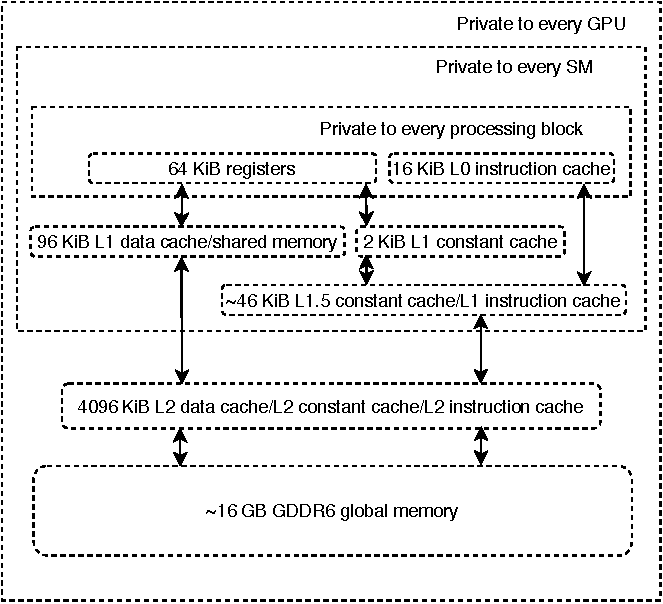
\includegraphics{figures/TeslaT4Mem.pdf}
    \caption{Nvidia Tesla T4 memory hierarchy~\cite{TeslaT4Bench}}
    \label{fig:t4_mem}
\end{figure}

\paragraph*{Memory hierarchy}
Any GPU incorporates several memory types, that serve different purposes and differ in access latency, size, and bandwidth.
The memory architecture of Tesla T4 is depicted in \ref{fig:t4_mem}.

\emph{Global memory} is the main resource to transfer data between host and device. It is the largest and the slowest memory space, cacheable in L1 and L2 caches, that have 32 B and 64 B lines respectively.
Global memory loads and stores by threads of a warp are served by the device with 32 B transactions\footnote{\url{https://docs.nvidia.com/cuda/pdf/CUDA\_C\_Best\_Practices\_Guide.pdf} (last accessed date: 30.05.2020)}.
Basically, concurrent accesses of the threads in a warp will coalesce into a number of such transactions necessary to service all the threads in the warp.
So in order to keep the number of such transactions to a minimum, threads in a warp should access adjacent segments of memory, aligned with the transaction size, avoiding strided accesses.
Such a requirement could not always be satisfied in practice, thus GPU resources being used not to its maximum. This memory space is accessible and allocated from the host, and visible to all the threads in a grid. 

\emph{Shared memory} is on-chip memory (hence it has lower latency and higher bandwidth than global memory) used to optimize frequent accesses to the same elements in global memory.
It is fast as long as bank conflicts do not occur.
The whole shared memory space is divided into 32 banks --- 4 B memory elements, with successive 4 B words belonging to successive banks. 
Any bank has a bandwidth of 4 B per clock cycle.
Therefore, any memory load or store of $n$ addresses, belonging to n distinct memory banks
could be serviced simultaneously with the bandwidth of $n$ times the bandwidth of a single bank.
However, accesses to memory addresses from the same bank are serialized, decreasing the effective bandwidth in a magnitude of the number of conflict-free accesses. When multiple threads of a warp access the same shared memory, a broadcast occurs. Several such broadcasts could coalesce into a single multicast. This memory space has a visibility scope of a single thread block and is not accessible from the host.

\emph{Constant memory} is a cacheable off-chip memory, that is read-only from the device. It is a 64 KB part of global memory, that has a specific path for caching. As a result, on a cache miss, a constant memory read costs one memory read from global memory; otherwise, it is as fast as register access. When the threads in a warp access different constant memory addresses, these accesses are serialized.  Thus the constant cache is best when the threads in warp access the same or very few distinct addresses, in the first case the access is broadcasted, and the latency is the same as registers one.

\emph{Register memory} is on-chip memory, consuming zero extra clock cycles per instruction, as long as there is no register read-after-write dependencies and bank conflicts. Is has a scope of a single thread and is the fastest memory type available.


\subsection{Memory optimizations}
Given such a sophisticated memory hierarchy that should be managed by a programmer, memory optimizations are in a great interest. Only automatic memory optimizations would be considered, avoiding the guidelines about how to rearrange existing access patterns and speed-up the transferring between host and device.

In cases when abundant data parallelism is hard to achieve, e.g. when utilizing concurrent data structures and related synchronization primitives that arbitrate the accesses, dynamic memory allocation, i.e. per-thread allocation inside the device code, for such data structures becomes a bottleneck, hurting the throughput. In~\cite{NvidiaAllocator} a novel approach for dynamic memory allocation is proposed. It is based on shared data structures, supporting fine-grained mutual exclusion regions, cooperative synchronization primitives allowing to allocate memory concurrently between the threads, and a policy of execution delegation. The proposed allocator has a much higher allocation throughput compared to the one, deployed with CUDA.

Since the register memory is bounded in size, excessive registers\footnote{When the compiler needs more registers, than available on SM.} could be spilled into the global memory, introducing higher latency. 
Contrary to the default CUDA compiler approach, that handles excessive registers via re-materialization\footnote{Recomputation of a value instead of loading and storing.
It produces the code with lower efficiency, however with lower register usage as well.} as long as possible before spilling, an approach from~\cite{RegisterSpilling} advocates the usage of underutilized shared memory to spill the excessive registers.
The approach is implemented as an extra binary translation pass over CUDA assembly.
Under certain conditions, such optimization is worse than CUDA default approach, thus the authors also provide a compile-time performance gain estimator, based on collected either explicit or implicit\footnote{Some stalls are labeled by the compiler, others are deduced, based e.g. on latencies for the memory type being accessed by the instruction.} instruction stalls, to compare the default code produced by the compiler and an optimized one, to decide which one is better.
On average, this technique achieves 10\% better performance on the selected benchmarks.

Another work is focused at the automatic allocation of shared memory to reduce the number of global memory transactions~\cite{AutomaticSharedMem} for automatically C-to-CUDA generated programs.
Authors propose a performance model, designed to choose the best configuration for shared memory allocation, considering estimated execution time, memory metrics, and the number of reduced global memory transactions.
Once the best configuration is found, it is applied
to the original C code by adding specific OpenACC\footnote{A set of directives for heterogeneous code parallelization} pragmas.

To tackle the problem of the lack of available GPU memory, a domain-oriented memory pooling and swapping is proposed in~\cite{zhang2019efficient}. Variables not in use are swapped to host and swapped back before any access, while variables that have non-overlapping lifetime could be allocated to the same memory space by the heuristic-driven memory pool. The heuristic is based on the iterative nature of the deep learning training algorithms to derive the lifetime and read/write order of all variables.

%тут бы переход какой-то к след подсекции
Despite such a variety of different memory optimization approaches, none of the presented works exploits possible static nature of device kernel parameters in any way. Thus, the application of partial evaluation technique to GPU kernels could provide another optimization approach, oriented at static data management.

\subsection{Partial evaluation}\label{PEsurvey}
%написать про partial evaluation с примером
\emph{Partial evaluation} is a program transformation and optimization technique, also known as program \emph{specialization}, first formulated in~\cite{Kleene1952-KLEITM}.
A partial evaluator is an algorithm, that takes a program and some of its known inputs called \emph{static} and produces another residual program, one yielding the same result given the remaining \emph{dynamic} inputs as the original program would have produced given all the inputs at once as illustrated in commutative diagram~\ref{fig:mix}.
A partial evaluator performs a mixture of code generation and execution: it reduces those parts of program \textbf{p}, depending on \textbf{in1}, and generates code for calculations for yet unavailable \textbf{in2}.
Generally, it performs symbolic computations, unfolding function calls, and replacement of function calls to their specialized versions.
For example, a partial evaluator for the program in listing~\ref{fig:pow} reduces the number of static conditional statements driven by static parameter. 

\begin{figure}
    \centering
    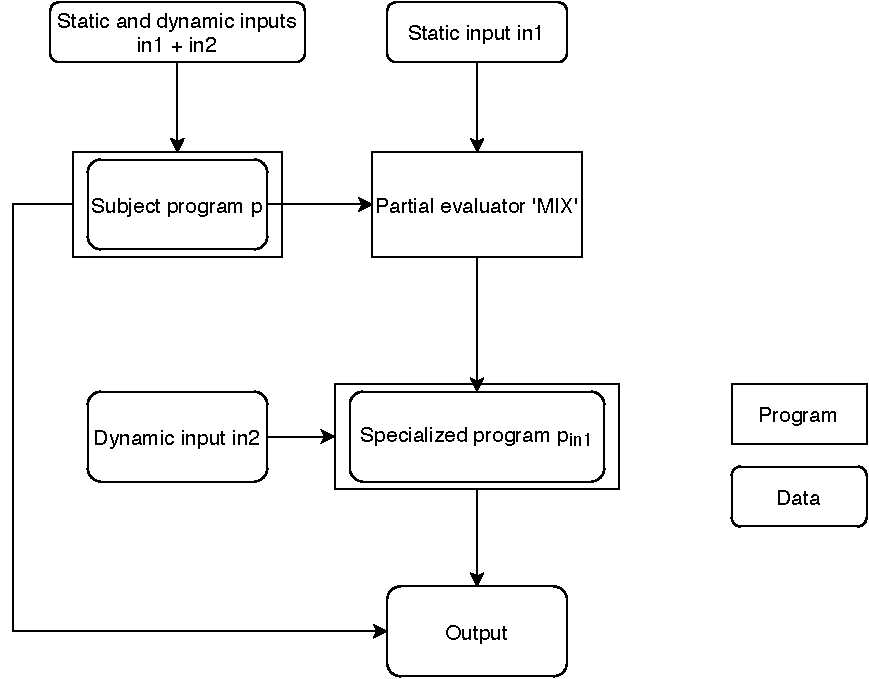
\includegraphics{figures/MixCommutativity.pdf}
    \caption{Partial evaluation pipeline}
    \label{fig:mix}
\end{figure}

The key idea is that a specialized program requires fewer computations (through moving them to compile or specialization time), and thus is intended to be more effective. A notable feature of specialization is the ability to generate a compiled program, once given an interpreter and a source program, also known as the first Futamura projection~\cite{Futamura1999}.
And while many practical applications benefit from partial evaluation through reducing the interpretation overhead (either by generating a compiler or exploiting interpretative nature of a program), there are scenarios, when a program takes more than one input, and one of the inputs varies more slowly than the others, thus specialization with respect to less-variable input could produce a more effective program.
Significant speed-up results were reported for pattern recognition, ray tracing, database querying, and scientific computing~\cite{Jones1993}.

\begin{code}[language=C,label=fig:pow,caption=Pow function partial evaluation example]
int pow(int x,int n){
    if (n == 0) return 1;
    else if (n \% 2 == 0) { 
        return pow2(f(x,n/2));
    }
    else return x * f(x,n-1);
}
//partially evaluating pow(x,5) would yield:
int pow(int x){
    return x * pow2(pow2(x));
}
\end{code}

In~\cite{JavaPe} an annotation-driven partial evaluator for Java programming language is introduced.
The goal is to specialize framework configurations and quite expensive reflection calls, which are widespread in object-oriented systems. The replacement of reflective method calls with partially evaluated ordinary calls allows to speed-up a dynamic pricing system by a power of six.

In~\cite{SuperVm} an approach for automatic virtual machine construction is proposed, which allows new languages to be implemented through the specification of abstract syntax tree interpreter. Partial evaluation is used to compile hot and stable parts of the already specialized\footnote{Supplied with runtime information such as types.} interpreter.

Another usage of partial evaluation as a means for compilation has been described in~\cite{LLVM-mix}. The PostgreSQL query interpreter, compiled at first to LLVM IR, which the designed partial evaluator works with, has been specialized in runtime with respect to the query, i.e. the query is compiled. The approach results in rather significant performance improvement, requires fewer efforts compared to just-in-time compiler development and is fully automatic.


Despite such a broad variety of partial evaluation- related research, at the moment of writing, there is a lack of research combining GPGPU and partial evaluation.
In~\cite{JitGPUPE} the approach from~\cite{SuperVm} was adopted to compile code from \emph{R} language to \emph{OpenCL}, to make it possible to write GPU-accelerated applications with dynamic interpreted languages, popular in big data, ignoring third-party libraries and relatively low-level programming languages for GPU. A metaprogramming system for writing shaders is presented in~\cite{GPUsh}, which supports partial evaluation via currying. However, the system is rather outdated and has no relation to modern GPGPU programming. Furthermore, there are no works dedicated to what benefits partial evaluation could provide once applied directly to GPU program, or whether it could provide any at all.

\begin{code}[language=Java,label=fig:kernel,caption=A typical GPGPU kernel]
handleData (filterParams, data)
{
  res = new List()
  for d in data
     for e in filterParams
        if d % e == 0
        then res.Add(d)
  return res
}
\end{code}


%$\llbracket \llbracket mix \rrbracket %[handleData,[2;3]]\rrbracket$
\begin{code}[language = Java, label = fig:kernel_mix,caption={ A typical GPGPU kernel specialization with respect to {[2;3]}}]
handleData (data)
{
  res = new List()
  for d in data
    if d % 2 == 0 ||
       d % 3 == 0
    then res.Add(d)
  return res
}
\end{code}

However, in practice, it appears that many GPGPU scenarios could have static parameters in a sense, theoretically appropriate for specialization.
A typical GPGPU kernel is depicted in listing~\ref{fig:kernel}.
It often represents some kind of a filter, that is applied to different pieces of the data in parallel by a huge number of threads.
The execution time primarily depends on the size of the data, which often exceeds the available memory of GPU, therefore the device kernel is run multiple times on different chunks of the data, resulting in significant execution time.
Hence, the filter varies less frequently than the data and could be considered as a static input and subjected to specialization.
However, the filter becomes known at runtime, before the kernel actually runs, thus the specialization should be performed at runtime.
The overhead of the partial evaluation could be hidden by the gained speed-up across the long run of the kernel.
Moreover, since one filter could be applied to different data pieces, the specialized version could be cached and reused instead of specializing again. The effect of specialization could be seen in listing~\ref{fig:kernel_mix}.
The inner cycle with accesses to the memory space of the filter has been reduced with the filter parameters being placed directly into the instructions.
Since memory access operations have been proven to be the most expensive, such a replacement could provide a benefit of accessing the filter from the registers, which is the fastest memory type, rather than from any other memory space.
Furthermore, a partial evaluator could be able to reduce those parts of the kernel, that depend on static filter parameters made available.

\subsection{AnyDSL framework}
To the date of writing, there is no partial evaluator known that works directly with CUDA C or any of CUDA intermediate representations.
As mentioned, the partial evaluator from~\cite{LLVM-mix} works with LLVM IR, and CUDA has an appropriate LLVM frontend, however, the partial evaluator leverages special attributes in IR, that conflicts with the ones of CUDA itself during LLVM JIT compilation.
AnyDSL~\cite{LeiBa} is a framework for the development of domain-specific libraries that could utilize different backends, including the one of CUDA.
The framework includes a partial evaluator that works with a specific intermediate representation, supporting CUDA C code generation.
The framework requires the programs to be developed in a special DSL named \emph{Impala}, which resembles C language with functions being the first- class objects.
Since the DSL is very CUDA C alike, the framework has been chosen as a means for partial evaluation of GPU programs.

The impala compiler translates the code into a functional graph-based intermediate representation similar to typed lambda calculus with continuations. Such a representation allows Impala to achieve near C performance, despite higher-order functions support~\cite{Thorin}.
Partial evaluation is performed on this level, while the representation could target different hardware architectures utilizing LLVM and compiler intrinsics.
An example of such an intrinsic is given in listing~\ref{impala_cuda}.
The whole function would be first converted into the intermediate representation, with the parts of the function labeled with \lstinline{@} partially evaluated, then the device-independent parts of the code would be translated into LLVM and device code would be translated into device-specific code, e.g. the code between lines 4-8 would be translated into CUDA C, which then would be included in LLVM code with a call to an external function that loads and executes the generated device code, e.g. the external function for mentioned lines would call NVIDIA CUDA compiler in runtime and launch the compiled kernel.

\begin{code}[language=Rust, label = impala_cuda, caption=Impala GPU-accelerated loop]
fn iterate(fld: Field , @body: fn(int, int) -> ()) -> () {
    let grid = (fld.cols , fld.rows , 1);
    let block = (128 , 1, 1);
    cuda(grid , block , || {
        let x = tid_x() + blockDim_x() * blockId_x();
        let y = tid_y() + blockDim_y () * blockId_y ();
        body(x, y);
    });
}
\end{code}

The authors of the framework evaluated the effectiveness of partial evaluation targeting different backends, including CUDA~\cite{LeiBa,OnlinePe}. The results show similar performance with hand-tuned third-party implementations. However, the authors focused on compile-time partial evaluation of kernels and have not provided any GPU-specific details that affect the success of the result as well as what particular optimization a partial evaluator performs with the device code. In contrast, this work is aimed at revealing GPU architecture details that affect the success of partial evaluation, focused at runtime partial evaluation and selects different experimental scenarios.


\section{Реализация библиотеки алгоритмов для полулокальных задач}\label{librarySection}
Как было отмечено в обзоре полулокальных задач,
существует необходимость в реализации большей части алгоритмов.
% В данном разделе будет описана реализация и архитектура библиотеки алгоритмов, связанных с полулокальными задачами.

% В качестве языка программирования был выбран \emph{Kotlin}

\subsection{Архитектура библиотеки}
В качестве языка программирования для написания библиотеки\footnote{https://github.com/NikitaMishin/SemiLocalLcs, дата обращения 26.05.2020} был выбран язык \emph{Kotlin}.


Код библиотеки можно  разделить на два логических модуля:
\begin{itemize}
    \item модуль \emph{semilocalProblem}  (рис.~\ref{fig:libraryProblem});
    \item модуль \emph{semilocalApplication} (рис.~\ref{fig:libraryApplication}).
\end{itemize}



\subsubsection{Модуль semilocalProblem}
В данном модуле реализована вся логика, отвечающая за задачи \emph{semi-local}.

% умножение муравья
Интерфейс \emph{IBraidMultiplication} отвечает за алгоритмы, реализующие операцию $\odot$, в частности, алгоритм \emph{муравья}.
В ходе работы алгоритма происходит последовательный доступ к перестановочным матрицам, к которым применен оператор $^{\nearrow}$ и $^{\swarrow}$\footnote{Оператор $^{\nearrow}$ ($^{\swarrow}$)  подсчитывает сумму элементов, которые лежат левее (правее) и ниже (выше) выбранного узла в матрице.}.
Для достижения быстрого времени доступа к элементам  матрицы ($O(1)$) используется
класс \emph{CountingQuery}, инкапсулирующий эту логику\footnote{Теорема 1 в \cite{tiskin2015fast}.}.
% 
Хранение перестановочных матриц реализовано с помощью хранения двух перестановок, отвечающим строчкам и столбцам матрицы.
Для реализации иной логики хранения необходимо реализовать методы абстрактного класса $AbstractPermuattionMatrix$

Классы, реализующие интерфейс \emph{ISemiLocalCombined}, инкапсулируют всю логику, связанную с задачей $semi-local$.
В частности, \emph{ImplicitSe-\\miLocalSA} инкапсулирует логику по неявному хранению матрицы, отвечающей задаче \emph{semi-local}, в виде \emph{ядра $P$} и соответствующими алгоритмами над ним.
На данный момент такими алгоритмами являются описанные в обзоре рекурсивный алгоритм с операцией $\odot$ и итеративный алгоритм распутывания кос.
Стоит отметить, что для быстрого доступа к произвольному элементу матрицы  используется интервальное двумерное дерево (\emph{range tree}), построенное над ненулевыми элементами ядра.
Это позволяет сократить объем требующейся памяти, но требует неконстантного времени доступа к элементам.
В случае если доступ последовательный, используется  \emph{CountingQuery}, который позволяет добиться константной асимптотической сложности.

\begin{figure}
    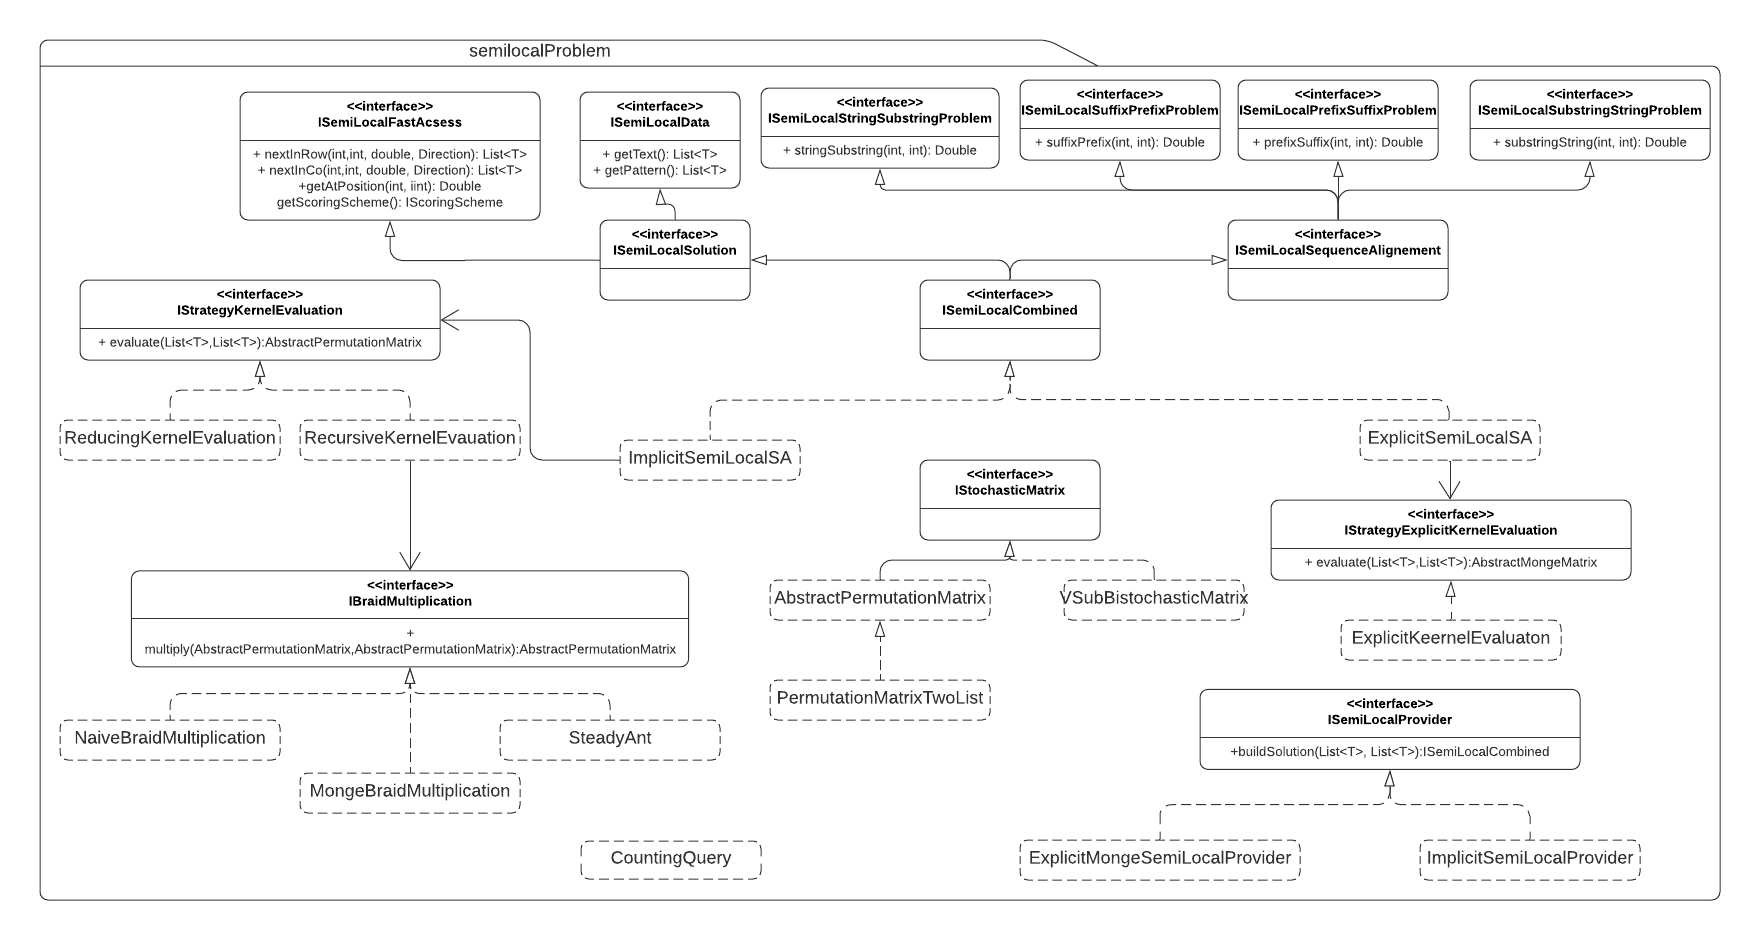
\includegraphics[height=0.72\columnwidth,angle=90]{figures/Library.png}
    \caption{Диаграмма классов UML части библиотеки, относящейся к различным задачам, основанным на  \emph{semi-local} задачах. Часть деталей и классов опущена.}\label{fig:libraryProblem}
\end{figure}

\emph{ExplicitSemiLocalSA} хранит матрицу $H_{a,b}$ в явном виде.
В данном случае нет экономии памяти, но доступ к произвольному элементу матрицы константный $O(1)$. 
Для решения задачи \emph{semi-local} используется алгоритм \emph{smawk}~\cite{aggarwal1987geometric}, отвечающий операции  $\otimes$.

% Стоит отметить, что недавние исследования~\cite{gawrychowski2020submatrix}, позволяют добиться 
% Нужно ли описать scorinSCheme



% \emph{ISemiLocalProvider}, \emph{ISemiLocalCombined} === паттерн фабричный метод
% набор классов и интерфейсов связанных с \emph{}
% Strategy --- стратегия




\subsubsection{Модуль semilocalApplication}
В данном модуле реализованы алгоритмы\footnote{Детальное описание алгоритмов и их доказательств находятся в ~\cite{tiskin2006all}}, для следующих задач:
\begin{enumerate}
    \item \emph{CompleteAMatch}
    \item \emph{Minimal-inclusive ThresholdAMatch}
    \item \emph{WindowAMatch}
    \item \emph{WindowSubstring}
    \item \emph{FragmentSubstring}
    \item \emph{BoundedLengthSmithWatermanAlignment}
\end{enumerate}

Первая задача относится к нахождению значения максимального выравнивания заданного шаблона $p$ и всех префиксов текста $t$ из всевозможных суффиксов из данного префикса:
\begin{equation}
    h[j] = \max _{i \in 0 ..j} sa(p,t[i,j]), j \in 0..|t|
\end{equation}

В рамках второй задачи ставится задача нахождения всех непересекающихся повторов шаблона $p$ в тексте $t$, чьи длины минимальны, а значение выравнивания выше заданного порога похожести $h$.

В третьей задаче необходимо найти все подстроки текста $t$ (уже могут пересекаться) длины $w$, чье выравнивание с шаблоном $p$ больше заданного порога похожести $h$.

Все эти три задачи сводятся к анализу \emph{подматрицы} задачи 
\emph{semi-local}, отвечающей \emph{srting-substring}.
И, соответственно, в зависимости от выбранного алгоритма решения задачи \emph{semi-local} асимптотика алгоритмов решения этих задач $O(n \times m \times \log n)$ и $O(v \times  m \times n)$.


\begin{figure}
    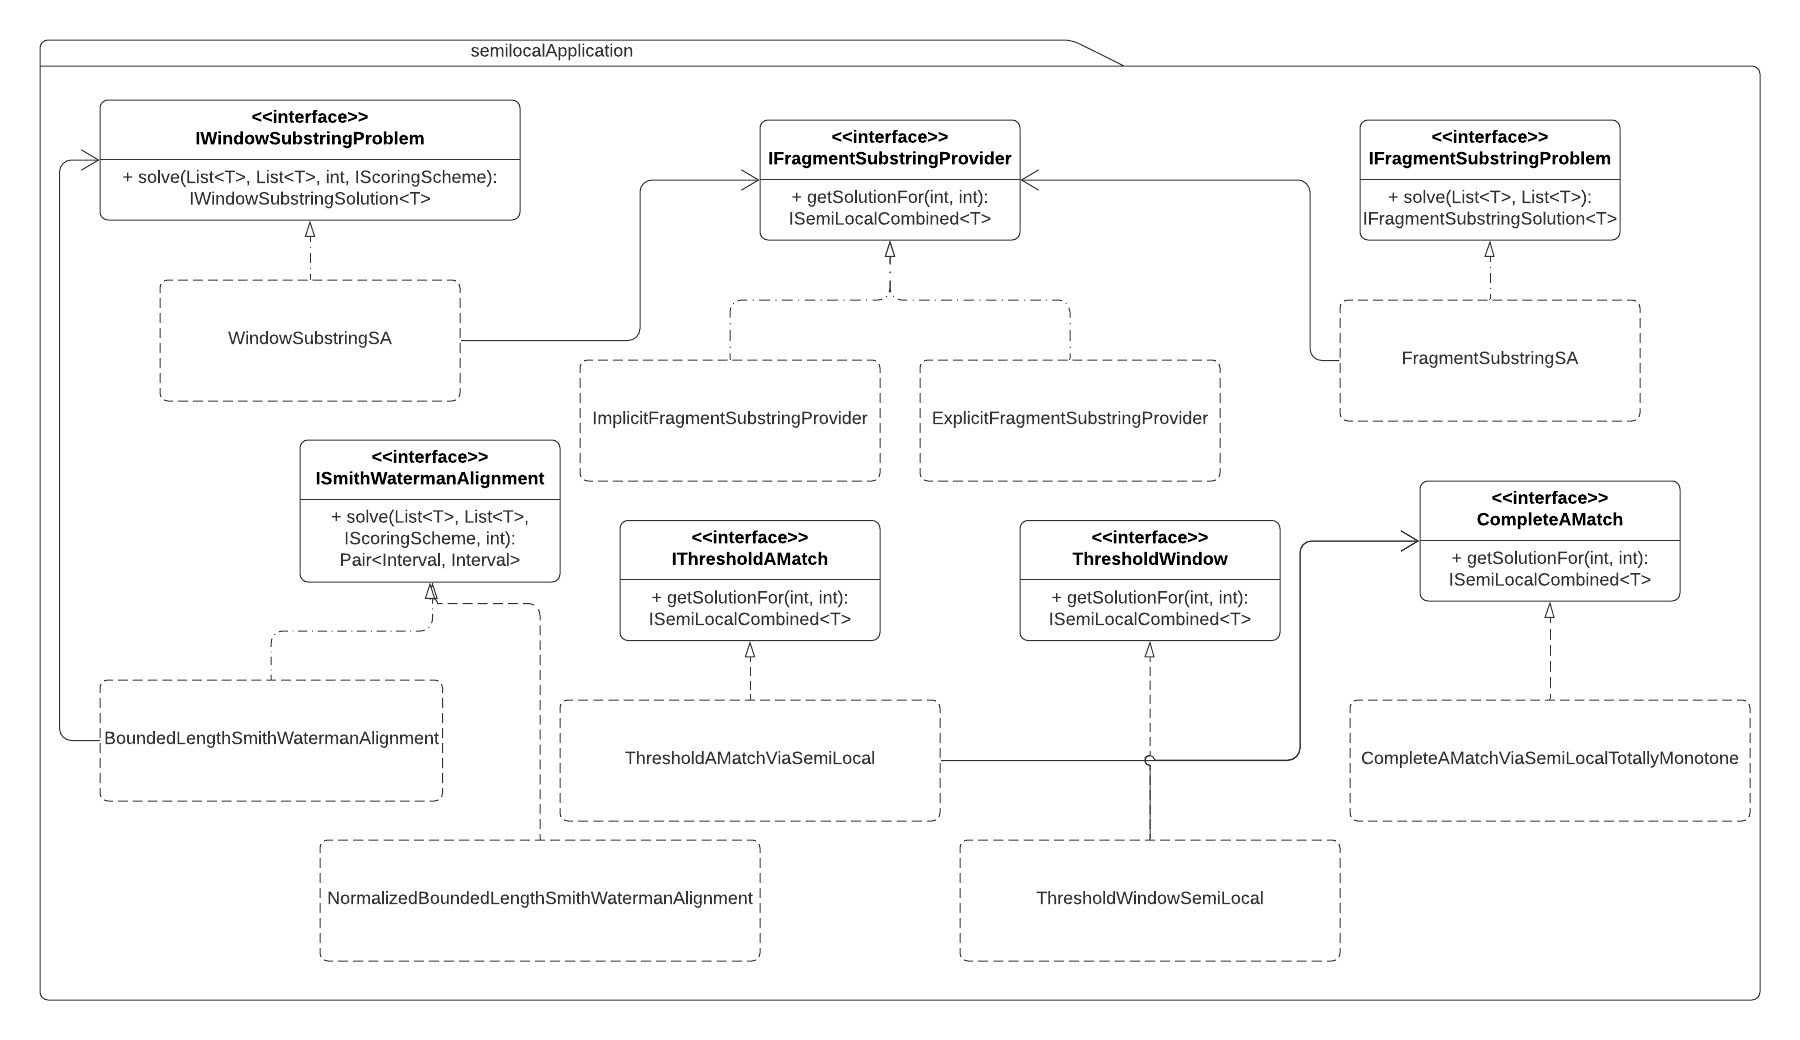
\includegraphics[width=\columnwidth]{figures/semiLocalApplication.png}
    \caption{Диаграмма классов UML части библиотеки, относящейся к \emph{semi-local} задачам. Часть деталей и классов опущена}\label{fig:libraryApplication}
\end{figure}


Задача \emph{FragmentSubstring} формулируется следующим образом: Для заданного множества интервалов (подстрок) $r$ из текста $t$ размера $m$ и текста $b$ размера $n$ необходимо вычислить \emph{semi-local} матрицу для каждого фрагмента из $r$ против $b$.
Имеет асимптотическую сложность $O(v^2 \times r \times  n \times \log m \times \log mv)$ \footnote{Существует возможность улучшить асиптотику до $O(v \times r \times  n \times \log^{2} m)$ } и $O(r \times n \times m  \times  log m)$.

Задача \emph{WindowSubstring}  является частным случаем   \emph{FragmentSubst-\\ring}, в которой размер фрагментов фиксирован.
Асимптотическая сложность решения уже будет $O(n \times m \times \log n)$ и $O(v^2 \times  m \times n)$.

Обе задачи основаны на двоичном разложении числа и предподсчете \emph{semi-local} решений, отвечающих данным разложениям.

Задача \emph{SmithWatermanAlignment} относится к локальному выравниванию.
В рамках данной задачи необходимо вычислить значение максимального локального выравнивания между $a$ и $b$, т.е найти пару подстрок, на которых достигается максимальное выравнивание.
Очень часто данная задача представляет интерес с различными ограничениями~\cite{arslan2004dynamic}.
Например, ограничения на минимальную длину подстрок.
Данное ограничение реализовано с помощью алгоритма из ~\cite{tiskin2019bounded} и инкапсулировано в соответствующем классе  \emph{BoundedLengthSmithWaterman-\\Alignment}.
Как отметил автор статьи, можно реализовать нормализованную версию данной задачи с применением \emph{BoundedLengthSmithWa-\\terman Alignment} к алгоритму из \cite{arslan2004dynamic}.

Нетрудно заметить, что часть алгоритмов в той или иной степени может быть адаптирована к задачам поиска повторов в документации.
Для задачи поиска по образцу такими кандидатами являются алгоритмы для решения задачи \emph{Minimal-inclusive ThresholdAMatch} и \emph{WindowSubstring}.
Для задачи поиска групп повторов могут быть применены  алгоритмы для \emph{WindowAMatch},
\emph{Minimal-inclusive ThresholdAMatch},\\\emph{BoundedLengthSmithWatermanAlignment} и \emph{semi-local}.

Адаптация алгоритмов к поиску повторов описана в следующем разделе.
Экспериментальная проверка асимптотики части алгоритмов, а так же их потенциальная возможность применения к большим данным даны в главе \ref{appob}.

% Соответствующая адаптация части алгоритмов описана в следующем разделе.

\section{Приложение для поиска повторов в документации ПО}\label{searchPO}
В данной главе  описано приложение для поиска повторов в документации ПО, в рамках которого будет производится экспериментальное исследование применимости алгоритмов, решающих полулокальные задачи.
Также описаны  основные технические решения и архитектура.
Описан подходы для поиска повтор.
Для каждой из \emph{задач поиска повторов} описано решение, основанное на использовании \emph{библиотеки алгоритмов} для полулокальных задач (см. главу \ref{librarySection}).

% Реализация приложения для поиска повторов в JavaDoc докумен-тации с применением алгоритмов решения полулокальных задач


\subsection{Общая архитектура приложения}
На рисунке \ref{fig:application} представлена архитектура приложения.
Оно реализовано в виде двух крупных компонент.

\begin{figure}[H]
    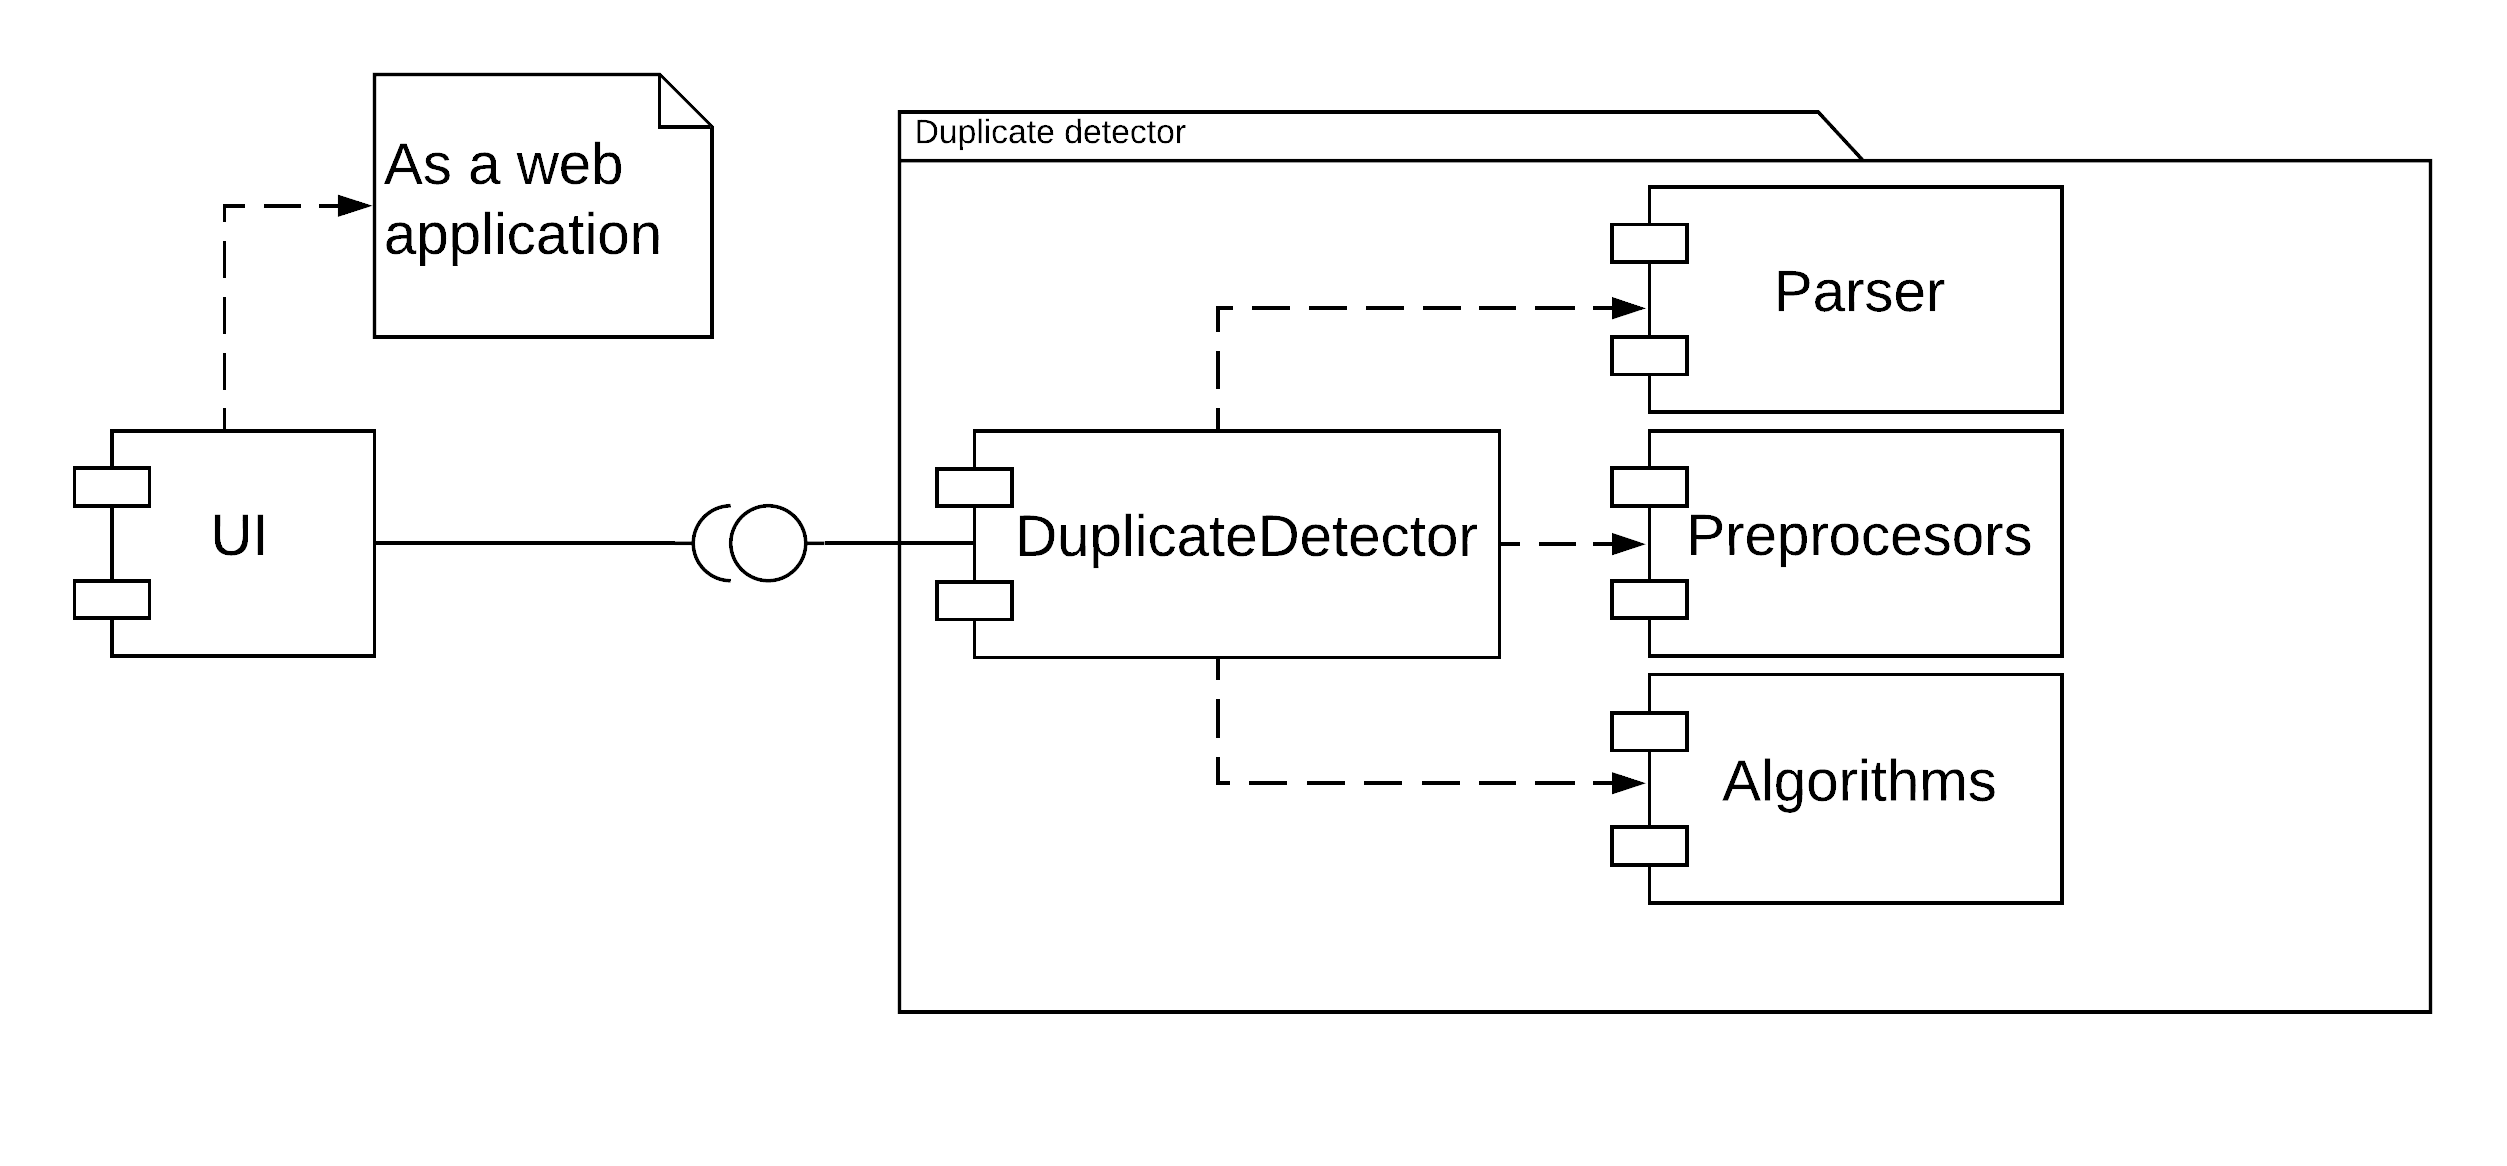
\includegraphics[width=\columnwidth]{figures/arhitecture.png}
    \caption{Диаграмма компонентов системы}\label{fig:application}
\end{figure}


Первая компонента (клиентская часть) --- это пользовательский интерфейс (\emph{UI}), который  отвечает за визуализацию и взаимодействие с пользователем.
Пользователь настраивает параметры поиска повторов, тип поиска, указывает файлы, в которых необходимо произвести анализ на дубликаты, или путь к проекту на \emph{Github} в интернете (рис. \ref{fig:startApp}).
Клиентская часть написана на \emph{python} и \emph{java script}.
Детальное описание клиентской части дано в секции \ref{clinet}.

Вторая компонента (серверная часть) отвечает за поиск повторов согласно заданным настройкам.
Данная часть написана на языке \emph{Kotlin}.
В секции \ref{server} детально описана функциональность данной части системы.

Взаимодействие между компонентами осуществляется посредством \emph{JSON}-формата.
Приложение реализовано в виде вэб-приложения, которое запускается в докер-контейнере, что минимизирует пользовательские требования для запуска программы\footnote{Достаточно иметь \emph{Docker} и \emph{Браузер}.}.

% Приложение реализовано в виде вэб-сервиса, который запускается в докер-контейнере на пользовательском компьюетере.



Стоит отметить, что в этой работе сделан основной акцент на поиск повторов в \emph{JavaDoc} документации в силу её актуальности для данного формата (см. главу \ref{duplicateReport}).

\begin{figure}[H]
    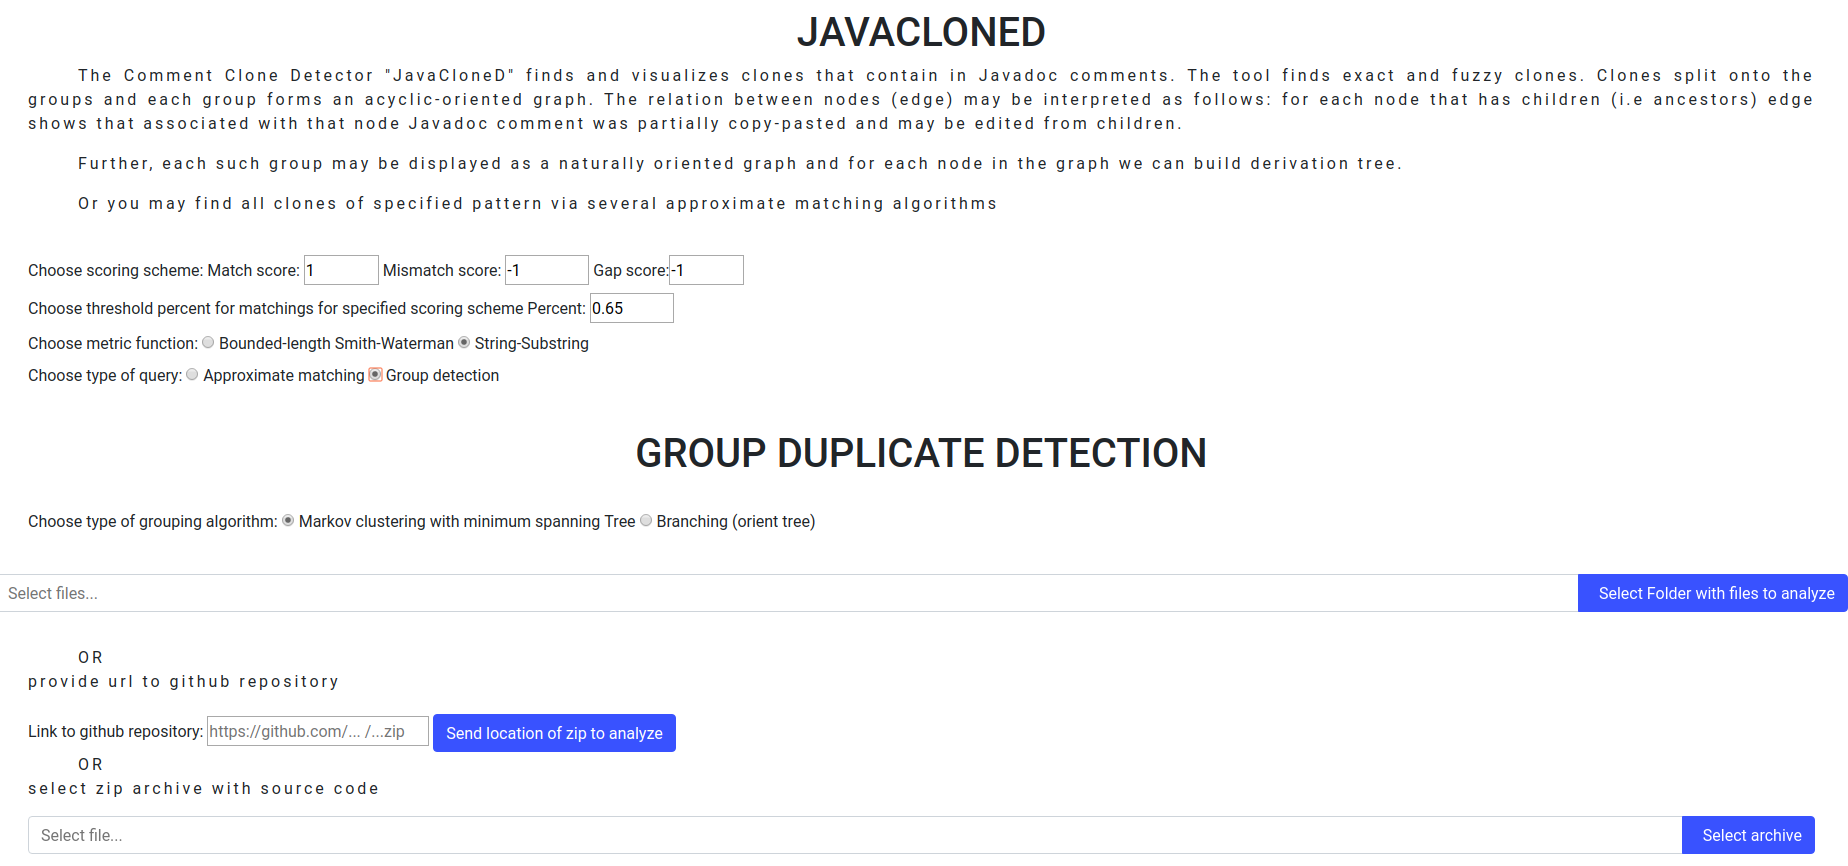
\includegraphics[width=\columnwidth]{figures/startApp.png}
    \caption{Интерфейс пользователя перед запуском анализатора для случая поиска групп повторов}\label{fig:startApp}
\end{figure}

\subsection{Клиентская часть}\label{clinet}
Как было отмечено выше, клиентская часть реализована в виде веб-приложения, которое написано посредством \emph{python}-фреймворка \emph{flask}\footnote{https://flask.palletsprojects.com/en/1.1.x/, микро-фреймворк для написания веб-приложений, дата обращения 26.05.2020}.
На основной странице вэб-приложения пользователь выставляет тип решаемой задачи, параметры запуска, указывает исходники и запускает вычисления.
Пользователь имеет возможность выбрать задачу \emph{"Поиск повтора по шаблону"} или \emph{"Поиск всех групп повторов"}.

Для визуализации найденных повторов в случае с  \emph{"Поиском повтора по шаблону"} результаты отображаются на странице ответа с цветовой расцветкой (см. рис. \ref{fig:pattViz}).


\begin{figure}[H]
    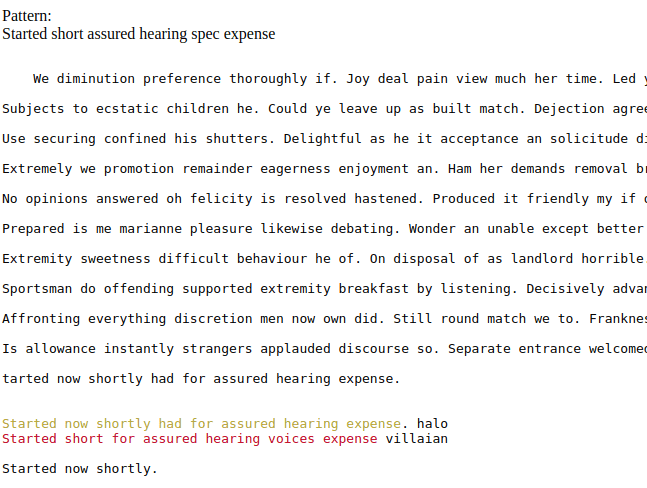
\includegraphics[width=\columnwidth]{figures/outputExampleAmatch.png}
    \caption{Визуализация найденных повторов для поиска по шаблону}\label{fig:pattViz}
\end{figure}

Для групп повторов механизм визуализации более комплексный (см. рис \ref{fig:groupViz}): используется три окна для интерпретации результатов.

\begin{figure}[H]
    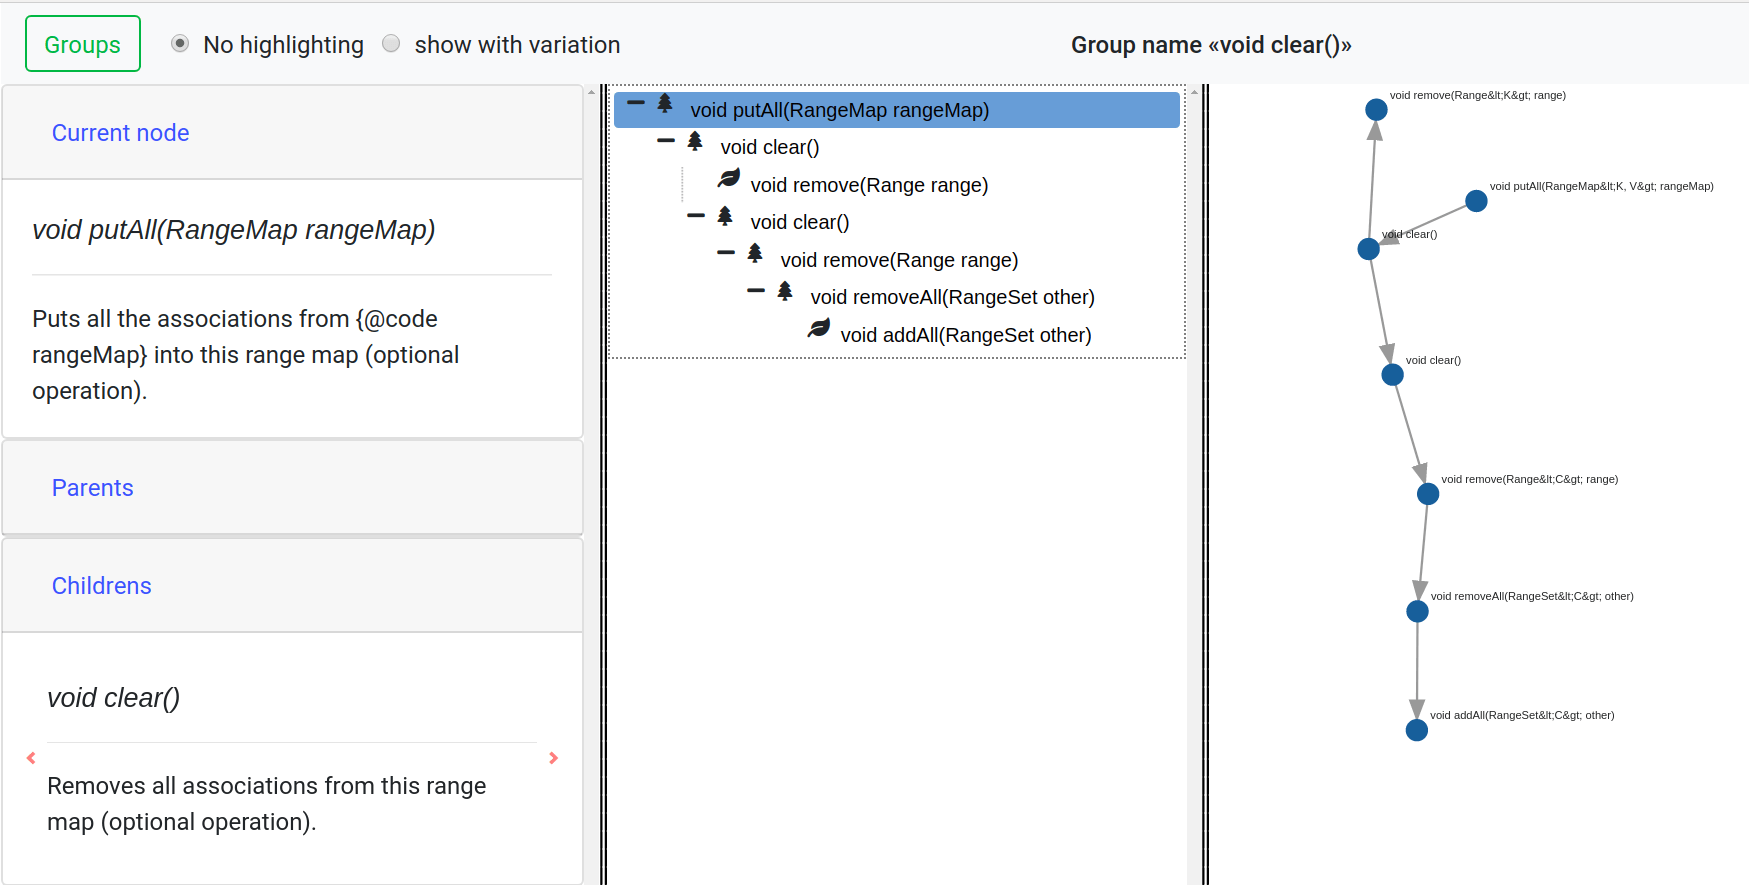
\includegraphics[width=\columnwidth]{figures/outputGroup.png}
    \caption{Визуализация групп повторов}\label{fig:groupViz}
\end{figure}


Первое окно отвечает за отображение отношений между фрагментами, которые состоят в отношении (имеют похожие части).
Интерпретация следующая: для текущего узла "родителем" являются все те фрагменты, в которые была взята часть информации с текущего фрагмента и, возможно, видоизменена.
"Детьми" являются те фрагменты, c которых, вероятнее всего, произошло дублирование информации.

Второе окно отвечает за представление каждого повтора в виде иерархической структуры.
Представление реализовано в виде \emph{tree control} --- для каждого повтора (вершины) строится ориентированное дерево вывода из этой вершины.
Такая интерпретация показывает, откуда вероятнее всего "произошел повтор", т.е откуда произошло дублирование данных.

Третье окно отвечает за визуализацию соответствующей группы повторов в  виде ориентированного графа.
Это позволяет увидеть структуру найденной группы. Все три окна синхронизированы между собой.

Описание используемых алгоритмов для нахождения повторов даны в секциях \ref{fics} и \ref{grouppa}  соответственно.    


% Рассмотрим пример работы  на рис \ref{TODO}. TODO описать пример. 

\subsection{Серверная часть}\label{server}
Как было указано выше, эта часть приложения отвечает за поиск повторов в документации.

На рис. \ref{fig:application} выделены компоненты серверной части (\emph{Kotlin application}).
Общий подход (\emph{pipeline}) поиска повторов заключается в следующем.

Сперва происходит синтаксический анализ с целью нахождения тех фрагментов, которые будут анализироваться согласно выбранным параметрам, заданными пользователем.
В данной работе анализируются \emph{JavaDoc} документация, а именно \emph{JavaDoc}-комментарии методов, классов и интерфейсов.
Это осуществлено с использованием библиотеки \emph{JavaParser}\footnote{https://javaparser.org/, дата обращения 26.05.2020}.
Для анализа иного вида документации (например, обычный текст, как в случае с поиском по образцу) достаточно в модуле \emph{Parser} реализовать необходимые интерфейсы.
Далее, комментарии обрабатываются различными фильтрами --- происходит токенизация, лемматизация, убираются стоп-слова и пр.


Данная обработка происходит с частичным использованием функциональности стэнфордского  фреймворка \emph{core nlp}\footnote{https://stanfordnlp.github.io/CoreNLP/, дата обращения 26.05.2020} для обработки естественного языка.

После этапа предобработки фрагментов происходит конвертация \\слов  в промежуточное представление в виде чисел с целью экономии памяти и ускорения работы алгоритмов.

Затем  происходит запуск соответствующих алгоритмов поиска, о которых пойдет речь дальше.


\subsection{Алгоритмы для решения задачи поиска повторов}\label{fics}
% fix

В данной секции будут описаны алгоритмы для решения задачи поиска по образцу, согласующиеся с определенной моделью в главе \ref{Model}.
Алгоритмы основаны на использовании \emph{библиотеки алгоритмов} (см. главу \ref{librarySection}).

\subsubsection{Улучшенный алгоритм интерактивного поиска}
В данной секции описана улучшенная версия алгоритма из \cite{luciv2019interactive}. Псевдокод алгоритма представлен ниже (алгоритм  \ref{alg:patternMathing1}).
\begin{algorithm}[H]
\caption{Нечеткий поиск по шаблону с использованием semi-local}\label{alg:patternMathing1}
Вход: шаблона поиска $p$, текст $t$, пороговое значение похожести $k$\\
Выход: множество непересекающихся повторов шаблона $p$\\
Комментарии:
\begin{equation}
    k_{di}=|p|*(\frac{1}{k}+1)(1-k^2)
\end{equation}
Псевдокод:
\begin{algorithmic}[1]
\State $W = semilocalSa(p,t)$
\State $W_2 = \emptyset$
\For{$w \in W$}
   \If{ $sa(p,w) \geq -k_{di}$}
   \State \emph{continue}
   \EndIf
   \State $maximums = FindMaxForColumnsBySmawk(w)$
   \State $max = FindMaxWithLenghtConstraint(maximums)$
   \If{$max \geq -k_{di}$}\Comment{В исходном был минимум, поэтому минус} 
    \State add substring associated with max to $W_{2}$ 
    \EndIf
\EndFor
\State $W_3 = UNIQUE(W_2)$\Comment{3 фаза без изменений}
\For{$w \in W_3$}
\If{$\exists w^{'} \in W_3:w \subset w^{'} $}
\State $remove$ $w$ $from$ $W_3$
\EndIf
\EndFor
\State $return$ $W_3$

\end{algorithmic}
\end{algorithm}

В строке $1$ вычисляется решение задачи \emph{semi-local sa}, в частности подзадачи \emph{string-substring}.
В строках ${3-12}$ внутри каждого окна размера $|w_{s}| \approx |p|$ сперва проверяется, что значение выравнивания шаблона $p$ и окна $w$ больше заданного порога похожести $k_{di}$, а затем внутри окна находится такая подстрока, что её выравнивания максимально среди всех друг подстрок данного окна. При одинаковом значении выравнивания будет выбираться наиболее длинная строка.
Строки ${13-18}$ отвечают фильтрации, в рамках которой происходит удаление одинаковых и пересекающихся повторов, в результате чего остаются только непересекающиеся повторы.

\paragraph*{Корректность улучшения}\mbox{}

Нетрудно заметить, что данная версия имеет лучшую асимптотическую сложность, чем исходный алгоритм. Более того, все свойства алгоритма сохраняются.

Исходный алгоритм разбит на 3 фазы: 'сканирование', 'усушка' и 'фильтрация'.

На первой фазе исходный текст $t$ анализируется скользящим окном размером $w_{s} = \frac{|p|}{k}$, где $k \in [\frac{1}{\sqrt{3}},1]$ параметр алгоритма, с шагом в один символ, а именно вычисляется редакционного расстояние\footnote{Метрика, минимальное количество операций вставки, удаления и замены одного символа на другой для превращения одной строки в другую.} между каждым окном и заданным шаблоном $p$.
Асимптотическая сложность данного шага $O(|p|^2 \times |t|)$ согласно \cite{luciv2019interactive}.

Заметим, что редакционное расстояние может быть выражено через выравнивание последовательностей.
Конкретнее, редакционное расстояние для данного случая выражается через следующую схему оценки:
\begin{equation}\label{weightAppr}
    (w_{+},w_{0},w_{-}) = (0,-2,-1)
\end{equation}
Соответственно, редакционное расстояние можно заменить на выравнивание последовательностей с весами $(0,-2,-1)$ и искать максимальное выравнивание без потери свойств алгоритма в силу эквивалентности двух задач.
Из этого следует, что можно применить алгоритмы для решения \emph{semi-local sa}.
В силу  формулы (\ref{weightNormalization}), значение нормализованной схемы будет следующее:
\begin{equation}
    (0, -2, -1) \rightarrow (1,\frac{\mu=0}{v=1}, 0)
\end{equation}
Таким образом, используя нормализацию, задачу можно свести к \emph{semi-local lcs}.
И, следовательно, асимптотическая сложность первой фазы алгоритма  из \cite{luciv2019interactive} может быть улучшена. Тогда её асимптотическая сложность будет $O(|t| \times |p|)$ вместо $O(|t| \times |p|^2)$.
Данная стадия эмулируется в строке $1$.

Во второй фазе происходит так называемая 'усушка' --- для каждого окна происходит вычисление минимальной подстроки, на которой достигается минимальное значение редакционного расстояния (в случае выравнивания последовательностей это относится к максимальному значению).
При равенстве расстояний выбирается подстрока наибольшая по длине.
Асимптотическая сложность данной фазы выражается как $O(|p|^4$).

Для улучшения данной фазы применяется следующее.
Матрица решений $H_{p,t}$ \emph{semi-local} содержит подматрицу \emph{string-substring}, которая содержит значения выравниваний шаблона $p$ со всеми подстроками текста $t$. 
Как было отмечено выше, эта матрица является анти-матрицей Монжа, следовательно, в ней можно быстро искать максимум в столбцах (строках) через алгоритм \emph{smawk}, имеющий асимптотическую сложность $O($\emph{размер матрицы}$\times$\emph{время доступа к элементу матрицы} = $\gamma$\footnote{Далее будет обозначать асимптотическую сложность доступа к произвольному элементу матрицы через символ $\gamma$}$)$.
Заметим, что этот алгоритм устойчив, в том плане, что он выдает первую позицию, на которой достигается максимум.
Например, если для текущего столбца $j$  максимум достигает в позициях $i$ и $i^{'}$, $i<i^{'}<=j$, то в результате работы \emph{smawk}, для столбца $j$ алгоритм выдаст $i$, что соответствует тому, что при равенстве значений будет выбираться наиболее длинная подстрока.
Имея максимумы для каждого столбца (каждого суффикса префикса), можно найти все максимумы и среди них выбрать подстроку наибольшую по длине.

Для нахождения максимума в столбце воспользуемся следующими соображениями.
\begin{itemize}
    \item  Если $H_{p,t}$ является \emph{анти-матрицей Монжа}, то $-H_{p,t}$ является \emph{матицей Монжа}.
    \item В результате транспонирования, матрица не перестает быть \emph{(анти)-матрицей Монжа}.
\end{itemize}
Иными словами, нахождение минимума в  строке в $-H_{p,t}^{T}$ будет соответствовать нахождению максимума в столбце в матрице $H_{p,t}$. 
В улучшенном алгоритме это отвечает строкам $7-10$.

Таким образом, асимптотическая сложность для каждого окна будет соответственно равна $O(|w_{s}| \times \gamma) $.
В худшем случае, таких окон будет $O(|t|)$.
Следовательно, вторая фаза алгоритма будет иметь асимптотическую сложность  $O(|w_{s}| \times |t| \times \gamma )$.
Учитывая то, что $k \in [\frac{1}{\sqrt{3}},1]$, то $|w_{s}| \approx |p|$ и $O(|w_{s}| \times |t| \times \gamma)=O(|p| \times |t| \times \gamma)$.
Значит, асимптотическая сложность второй фазы $O(|p| \times |t| \times \gamma )$, все свойства алгоритма сохранены.

Третья фаза, отвечающая за фильтрацию фрагментов, остается без изменений. Ее асимптотическая сложность $O(|p| \times \log |p|)$ согласно \cite{luciv2019interactive}.

Соответственно, алгоритм сохранит все свои свойства и будет уже иметь асимптотику $O(|p| \times |t|)$\footnote{В то время как исходный алгоритм оценивается как $\max (O(|p|^2 \times |t|, O(|p|^4)$, что при $|p| \approx |t|$ дает 4 степень.}.
Заметим, что алгоритм имеет оптимальную асимптотику при явном хранении матрицы $H_{p,t}$ (время доступа к произвольному элементу константное) согласно \cite{abboud2015tight}.
% Как отмечено выше, псевдокод алгоритма представлен на  \ref{alg:patternMathing1}.

\subsubsection{Алгоритм нечеткого поиска шаблона с использованием ThresholdAMatch}
Более простое решение относится к алгоритму \ref{alg:patternMathing2}, реализация которого уже содержится в \emph{библиотеке алгоритмов}. 
Он позволяет найти все непересекающиеся повторы шаблона $p$ в тексте $t$.

\begin{algorithm}[h]
\caption{Нечеткий поиск по шаблону с использованием Min-inclusive ThresholdAMatch}\label{alg:patternMathing2}
Вход: шаблона поиска $p$, текст $t$, пороговое значение похожести $h$\\
Выход: множество непересекающихся повторов шаблона $p$\\
Комментарии: в реализации $h$ высчитывается исходя из схемы оценки и процента похожести, выраженного через число из отрезка $[0,1]$\\
Замечание: При использовании интервального дерева данный алгоритм можно адаптировать таким образом, что на каждом шаге будет выбираться максимальный интервал из текста.
Тогда асимптотика возрастет в $O(log|t|)$ раз\\
Псевдокод:
\begin{algorithmic}[1]
\State $maxSuffixes= CompleteAMatch(p,t)$
\State $reverse(maxSuffixes)$
\State $result = \emptyset$
\For{$(i,j,score) \in maxSuffixes$}
   \If{$score \geq h \& j \leq res.last().i $} 
    \State $res.add((i,j,score))$ 
    \EndIf
\EndFor
\State $return$ $result$

\end{algorithmic}
\end{algorithm}

Сперва решается задача \emph{CompleteAMatch}, в рамках которой для каждого столбца $j$ подматрицы \emph{string-substring} находится максимальное значение и позиция $(i,j')$, в которой оно  достигается, т.е находится суффикс префикса, который больше всего похож на шаблон.
Далее, над полученным результатом производится фильтрация, начиная с конца.
В результате чего остаются только непересекающиеся повторы минимальной длины, которые больше заданного порога похожести.
Асимптотическая сложность данного решения зависит от выбранного алгоритма  решения \emph{semi-local}.
Соответственно, $O(|t| \times |p| \times \log |t|)$, $O(|t| \times |p| \times v^2)$ или $O(|t| \times |p| \times v)$.

Данный алгоритм рассматривается как альтернатива алгоритму \ref{alg:patternMathing1}.

\subsubsection{Алгоритм нечеткого поиска шаблона с использованием Разреза}

Еще одним решением на основе \emph{semi-local} является следующий алгоритм.
Во-первых, задачу поиска по шаблону можно сформулировать с иной точки зрения: 
необходимо найти все максимальные по выравниванию непересекающиеся повторы шаблона $p$ в тексте $t$, т.е получить такую цепочку непересекающихся интервалов $(i_1,j_1),...,(i_n,j_n)$, что на $(i_k,j_k)$ достигается максимальная похожесть на еще непокрытой найденными интервалами части текста $t$.
В рамках задач \emph{semi-local} это означает разбитие матрицы \emph{string-substring} на непересекающиеся подматрицы, с учетом максимумов в подматрицах.
Последнее относится к быстрому поиску максимума в матрице (\emph{range maximum query}).
В силу того, что матрица \emph{string-substring} является матрицей Монжа, можно применить результат из статьи  \cite{gawrychowski2020submatrix}. 
Для этого необходимо реализовать структуру данных, асимптотическая сложность построения которой равна $O(|t|\times \log |t|)$ (размер структуры выражается как $O(|t|)$), которая позволяет делать запросы на поиск максимума в произвольной подматрице, имеющие асимптотическую сложность $O(\log \log|t|)$.
Учитывая, что непересекающихся повторов в тексте $t$ может быть в худшем случае $|t|$ штук,
для их нахождения необходимо осуществить $|t|$ запросов на поиск максимуму.
Следовательно, конечная асимптотика алгоритма $O(|t| \times \log \log t) +O($\emph{сложность подсчета 
semi-local}$)=O($\emph{сложность подсчета 
semi-local}$)$, так как $\log \log |t| \leq |p|$ для достаточно больших значений $|t|$. 
Псевдокод алгоритма представлен на листинге \ref{alg:patternMathing3}.

\begin{algorithm}[h]
\caption{Нечеткий поиск по шаблону с использованием maxRangeQuery}\label{alg:patternMathing3}
Вход: шаблон поиска $p$, текст $t$, пороговое значение похожести $h$\\
Выход: множество непересекающихся повторов шаблона $p$\\
Комментарии: в реализации $h$ высчитывается исходя из схемы оценки и процента похожести, выраженного через число из отрезка $[0,1]$\\
Псевдокод:
\begin{algorithmic}[1]
\State $S = SolveSemiLocalSA(p,t)$
\State $W = BuildStructForRangeQuery(S)$
\State $IntervalsToSearch = \emptyset $
\State$IntervalsToSearch.add((0,|t|))$
\State $result = \emptyset$
\While{$IntervalsToSearch.isNotEmpty()$}
    \State $(i,j) = IntervalsToSearch.pop()$
    \State $score,i^{'},j^{'} = W.query(i,j)$
    \If{$score \geq h $} 
    \State $result.add(( i^{'},j^{'},score ))$
    \State $IntervalsToSearch.add(i,i^{'})$        \State $IntervalsToSearch.add(j^{'},j)$
    \EndIf
\EndWhile
\State $return$ $result$

\end{algorithmic}
\end{algorithm}


% Для апробации применимости \emph{semi-local} было решено реализовать алгоритм \ref{alg:patternMathing2} т.к
% для \ref{alg:patternMathing1} была произведена апробация в статье \cite{luciv2019interactive}, а \ref{alg:patternMathing3} на данный момент не имеет доказанных теоретических свойств и требует использования сложной структуры данных из \cite{gawrychowski2020submatrix}.

% Для задачи поиска по образцу постпроцессинг не нужен.

\subsection{Алгоритмы для решения задачи поиска групп повторов}\label{grouppa}
В данной главе описаны алгоритмы решения задачи поиска групп повторов на основе использования \emph{библиотеки алгоритмов} и применения графовых алгоритмов.

Согласно определенной в секции \ref{Model} модели, для решения задачи \emph{поиска групп повторов}  необходимо
задать функцию похожести $g$ и выбрать предикат $\gamma$.
Заметим, что для рассматриваемого случая, текстовыми фрагментами, в которых ищутся повторы, являются цельные \emph{JavaDoc}-комментарии.
Соответственно, в данной работе в отношении поиска групп повторов \emph{повторами} будут служить семантически замкнутые куски текста, как и в \cite{soto2015similarity}\footnote{В \cite{soto2015similarity} это были топики текста в \emph{Dita} документации.}, т.е \emph{JavaDoc} комментарии.

Соответственно, весь набор комментариев образует граф.
Он может быть как ориентированным, так и неориентированным.
Это зависит  от того, является ли $g$ симметричной по отношению к своим аргументам.
Таким образом, в полученном графе можно выделить группы повторов согласно предикату $\gamma$.
На \ref{alg:groupDuplicate} представлен псевдокод алгоритма.
Отметим, что асимптотика алгоритма выражается, как $\max (O(|t|^2*g), O(s))$.

Функция $g$ может быть определена через локальное, полулокальное и глобальное выравнивание, соответственно.
В данной работе в качестве $g$ выбраны следующие алгоритмы из \emph{библиотеки алгоритмов}.
\begin{itemize}
    \item \emph{BoundedLengthSmithWaterman} --- локальное выравнивание.
    % , симметричная функция.
    \item \emph{Semi-local sa} --- полулокальное выравнивание.
    % не симметричная функция.
    % \item \emph{ThrehsoldAMatch} --- поиск по шаблону. 
\end{itemize}

\begin{algorithm}[h]
\caption{Алгоритм поиска групп повторов для JavaDoc-комментариев}\label{alg:groupDuplicate}
Вход: набор комментариев $t_{i}$, функция $g$, которая меряет похожесть между двумя комментариями, функция $s$, которая согласно выбранному предикату $\gamma$ строит группы, пороговое значение похожести $h$\\
Выход: группы непересекающихся повторов\\
Комментарии: в реализации $h$ высчитывается исходя из схемы оценки и процента похожести, выраженного через число из отрезка $[0,1]$\\
Псевдокод:
\begin{algorithmic}[1]
\State $graph = Graph(vertices=t)$
\For{$t_{i} \in t $}
\For{$t_{j} \in t,t_{i} \neq t_{j} $}
\If{$g(t_{i},t_{j})\geq h $}
\State $addEdge(t_{i},t_{j},g(t_{i},t_{j}))$
\EndIf
\If{$g(t_{j},t_{i}) \geq h$}
\State $addEdge(t_{j},t_{i},g(t_{j},t_{i}))$
\EndIf
\EndFor
\EndFor
\State $groups = s(graph)$
\State $return$ $groups$
\end{algorithmic}
\end{algorithm}

% На \ref{1,2,3} представлены алгоритмы, определяющие функцию $s$

Следующие эвристические соображения помогают определить функции $s$, которые подходят для нахождения групп.

Во-первых, в силу того, что мы рассматриваем граф, естественным образом задача сводится к  кластеризации графа/выделению компонент (сильной) связности.

Во-вторых, ориентированное ребро $a \xrightarrow{g(a,b)} b$ в графе можно естественным образом интерпретировать так: часть текста из $b$ была скопирована в фрагмент $a$ или текст $b$ был скопирован, и в новом фрагменте произведена модификация этой копии и получено $a$.
При существовании обратного ребра будем считать, что при условии $g(a,b)\geq g(b,a)$, $a$ является потомком $b$ (помним, что в общем случае $g(a,b)\neq g(b,a)$ и наоборот.

В-третьих, очень часто бывает, что повторы практически не отличаются друг от друга или же в точности совпадают друг с другом.
Такие повторы хочется различать от обычных.
Если рассматривать граф, такое состояние для части вершины выражается через термин \emph{клика}\footnote{Полный граф на заданных вершинах.} и относится к задаче поиска клики.
Соответственно, новый граф, в котором присутствуют клики строится, из исходного обновлением весов тех ребер, которые входят в клики или находятся внутри клик.


В-четвертых, ассоциированный с группой ориентированный граф должен быть деревом.
Эта эвристика основана на том, что вершина не может быть потомком сама себе (наличие циклов) и не может иметь двух одинаковых потомков (проблема множественного наследования).
Соответственно, граф является деревом.  

Исходя из описанных выше эвристик, были разработаны алгоритмы \ref{alg:cluster1}, \ref{alg:clusterMcl}.
Также применен алгоритм из статьи \cite{tofigh2009optimum}.

% 
В \ref{alg:cluster1} используется идея иерархической кластеризации с тем изменением, что добавляется новый вид вершины, который олицетворяет клики.
Как известно, поиск клики --- это \emph{NP}-полная задача.
Поэтому в данном алгоритме произведена аппроксимация поиска клик:
листовая вершина принадлежит кластерному узлу, если её  расстояние до клики больше заданного порога похожести для клик.
% \red{Для подсчета расстояний будет использоваться \emph{минимальное расстояние между вершинами}.} 
% Существует разные варианты подсчета расстояний, о них подробно  будет описано в главе TODOапробации.
В ходе алгоритма в цикле \emph{while} происходит нахождение двух ближайших вершин согласно выбранной метрике, их объединение согласно правилам и пересчет матрицы расстояний, которая отвечает уже новому графу.
В общем случае\footnote{Некоторые метрики позволяют считать асимптотически быстрее.} пересчет матрицы требует $O(n^2)$ времени, где $n$ --- количество вершин.
В худшем случае  цикл \emph{while} будет исполняться $O(n)$ раз,
тогда асимптотика алгоритма составит $O(n^3)$.
% песос пример нужен лучше напиши епта

% иерархичпская кластеризация
\begin{algorithm}[h]
\caption{Алгоритм выделения групп на основе Иерархической кластеризации}\label{alg:cluster1}
Вход: граф $G$ с матрицей расстояний, функция  $f$, которая считает дистанцию между вершинами, пороговое значение похожести $h_{clique}$, при котором вершины образуют очередной уровень в иерархии, $h_{group}$ --- пороговое значение похожести\\
Выход: иерархические группы повторов \\
Псевдокод:
\begin{algorithmic}[1]
\State $roots = G.vertices()$
\While{$roots.isNotEmpty()$}
\State $(from, to,score) = closestVertices(root)$
\State $newVertex = switch \{$
\State $score\geq h_{clique} , from,to \in Leaf \rightarrow Clique(from,to) $
\State $score\geq h_{clique} , to \in Clique,from \in Leaf \rightarrow to.add(from);to $
\State $score\geq h_{clique} , from,to \in Clique \rightarrow from.addAll(to);from$
\State $score\geq h_{group}, \rightarrow ClusterNode(from,to) $
\State $else \rightarrow break$ 
\State $\}$
\State $G.recalcualateDistance()$
\State $roots.remove(from)$
\State $roots.remove(to)$
\State $roots.add(newVertex)$
\EndWhile
\State $return$ $roots$
\end{algorithmic}
\end{algorithm}

В алгоритме \ref{alg:clusterMcl} использована идея кластеризации на основе марковских моделей~\cite{dongen2000cluster} и дальнейшего построения минимальных остовных деревьев внутри каждого кластера.
 Асимптотическая сложность первого шага реализации в данной работе $O(n^3)$ в худшем случае.
 Нахождение минимального остовного дерева реализовано с помощью алгоритма Крускала с использованием системы непересекающихся множеств. Сложность второго шаге $O(n^2 \times \log n)$.
 Соответственно, общая сложность $O(n^3)$.

% mcl clustering
\begin{algorithm}
\caption{Алгоритм выделения групп на основе Марковских моделей}\label{alg:clusterMcl}
Вход: граф $G$ с матрицей расстояний\\
Выход: группы повторов с структурой группы в виде дерева\\
Псевдокод:
\begin{algorithmic}[1]
\State $trees = \emptyset$
\State $ clusters = mclClustering(G)$
\For{$cluster \in clusters$}
\State $tree =  BuildMaximumSpanningTree()$
\State $trees.add(tree)$
\EndFor
\State
\State $return$ $trees$
\end{algorithmic}
\end{algorithm}


Алгоритм \cite{tofigh2009optimum}  решает задачу построения такого ориентированного подграфа $G_{branch}$ из исходного $G$, что:
\begin{itemize}
    \item В нем нет циклов
    \item Ни в какую вершину не входит больше одного ребра
\end{itemize}
Причем среди всех таких подграфов он оптимален:
\begin{equation}
\sum_{w \in G_{branch}} w \geq \sum_{w^{'} \in G_{branch^{'}}} w^{'}
% \forall G_{branch^{'}} 
\end{equation}
Это соотносится с последней эвристикой о том, что граф должен быть деревом.
Алгоритм из \cite{tofigh2009optimum} обладает асимптотической сложностью $O(n^2)$.

% вероятностная кластеризация
% разбить компоненты сильной связности-> построить ориентированное дерево
%  

\vspace{10 mm}
Результаты применимости описанных алгоритмов из  данной главы к поиску повторов в документации ПО представлены в разделе \ref{appob}.
\section{Evaluation}

We evaluate the implemented algorithm on both regular and context-free path queries in order to demonstrate applicability of the proposed solution.
Namely, goals of the evaluation are following.
\begin{enumerate}
	\item Investigate the practical applicability of RPQ evaluation by the proposed algorithm.
	\item Compare Azimov's algorithm for reachability CFPQ and the proposed algorithm.
	\item Investigate the practical applicability of paths extraction algorithm for both regular and context-free queries.
\end{enumerate}

For evaluation, we use a PC with Ubuntu 18.04 installed.
It has Intel core i7-6700 CPU, 3.4GHz, and DDR4 64Gb RAM.
As far as we evaluate only algorithm execution time, we store each graph fully in RAM as its adjacency matrix in sparse format.
Note, that graph loading time is not included in the result time of evaluation.	

\subsection{RPQ Evaluation}

In oder to investigate applicability of the proposed algorithm for RPQ over real-world graphs we collect a set of real-world and synthetic graphs and evaluate queries generated by using the most popular templates for RPQs.

\subsubsection{Dataset}

Brief description of collected graphs are presented in Table~\ref{tbl:graphs_for_rpq}.
Namely, the dataset consists of several parts.
The first one is a set of LUBM graphs\footnote{Lehigh University Benchmark (LUBM) web page: \url{http://swat.cse.lehigh.edu/projects/lubm/}. Access date: 07.07.2020.}~\cite{10.1016/j.websem.2005.06.005} with a different number of vertices.
The second one is a graphs from Uniprot database\footnote{Universal Protein Resource (UniProt) web page: \url{https://www.uniprot.org/}. All files used for evaluation can be downloaded here: \url{ftp://ftp.uniprot.org/pub/databases/uniprot/current_release/rdf/}. Access date: 07.07.2020.}: \textit{proteomes}, \textit{taxonomy} and \textit{uniprotkb}.
The last part is a RDF files \textit{mappingbased\_properties} from DBpedia\footnote{DBpedia project web site: \url{https://wiki.dbpedia.org/}. Access date: 07.07.2020.} and \textit{geospecies}\footnote{The Geospecies RDF: \url{https://old.datahub.io/dataset/geospecies}. Access date: 07.07.2020.}.
These graphs represent data from different areas and they are frequently used for graph querying algorithms evaluation.

\begin{table}
{
\rowcolors{2}{black!2}{black!10}
\begin{tabular}{|l|c|c|}
\hline
Graph & \#V & \#E \\
\hline
\hline 
LUBM1k  & 120 926 & 484 646 \\
LUBM3.5k  & 358 434 & 144 9711 \\
LUBM5.9k  & 596 760 & 2 416 513 \\
LUBM1M   & 1 188 340 & 4 820 728 \\
LUBM1.7M & 1 780 956 & 7 228 358 \\
LUBM2.3M & 2 308 385 & 9 369 511 \\
\hline
Uniprotkb & 6 442 630 & 24 465 430 \\
Proteomes & 4 834 262 & 12 366 973 \\
Taxonomy & 5 728 398 & 14 922 125 \\
\hline
Geospecies & 450 609 & 2 201 532 \\
Mappingbased\_properties & 8 332 233 & 25 346 359 \\
\hline
\end{tabular}
}
\caption{Graphs for RPQ evaluation}
\label{tbl:graphs_for_rpq}
\end{table}


Queries for evaluation was generated by using templates of the most popular RPQs which are collected from~
\cite{Pacaci2020RegularPQ} (Table 2) and~\cite{Wang2019} (some of complex queries from Table 5), and are presented in table~\ref{tbl:queries_templates}.
We generate 10 queries for each template and each graph using the most frequent relations from the given graph randomly\footnote{Used generator is available as part of CFPQ\_data project: \url{https://github.com/JetBrains-Research/CFPQ_Data/blob/master/tools/gen_RPQ/gen.py}. Access data: 07.07.2020.}. 
For all LUBM graphs common set of queries was generated in order to investigate scalability of the proposed algorithm.

\begin{table}
{\small
\renewcommand{\arraystretch}{1.25}
\rowcolors{2}{black!2}{black!10}
\begin{tabular}{|c|c||c|c|}
\hline

Name & Query & Name & Query \\
\hline
\hline 
$Q_1$   & $a^*$                               & $Q_9^5$    & $(a \mid b \mid c \mid d \mid e)^+$                     \\
$Q_2$   & $a\cdot b^*$                        & $Q_{10}^2$ & $(a \mid b) \cdot c^*$                                  \\
$Q_3$   & $a \cdot b^* \cdot c^*$             & $Q_{10}^3$ & $(a \mid b \mid c)  \cdot d^*$                          \\
$Q_4^2$ & $(a \mid b)^*$                      & $Q_{10}^4$ & $(a \mid b \mid c \mid d)  \cdot e^*$                   \\
$Q_4^3$ & $(a \mid b \mid c)^*$               & $Q_{10}^5$ & $(a \mid b \mid c \mid d \mid e)  \cdot f^*$            \\
$Q_4^4$ & $(a \mid b \mid c \mid d)^*$        & $Q_{10}^2$ & $a \cdot b$                                             \\
$Q_4^5$ & $(a \mid b \mid c \mid d \mid e)^*$ & $Q_{11}^3$ & $a \cdot b \cdot c$                                     \\
$Q_5$   & $a \cdot b^* \cdot c$               & $Q_{11}^4$ & $a \cdot b \cdot c \cdot d$                             \\
$Q_6$   & $a^* \cdot b^*$                     & $Q_{11}^5$ & $a \cdot b \cdot c \cdot d \cdot f$                     \\
$Q_7$   & $a \cdot b \cdot c^*$               & $Q_{12}$   & $(a \cdot b)^+ \mid  (c \cdot d)^+$                     \\
$Q_8$   & $a? \cdot b^*$                      & $Q_{13}$   & $(a \cdot(b \cdot c)^*)^+ \mid  (d \cdot f)^+$          \\
$Q_9^2$ & $(a \mid b)^+$                      & $Q_{14}$   & $(a \cdot b \cdot (c \cdot d)^*)^+  \cdot (e \mid f)^*$ \\
$Q_9^3$ & $(a \mid b \mid c)^+$               & $Q_{15}$   & $(a \mid b)^+ \cdot (c \mid d)^+$                       \\
$Q_9^4$ & $(a \mid b \mid c \mid d)^+$        & $Q_{16}$   & $a \cdot b \cdot (c \mid d \mid e)$                     \\
\hline
\end{tabular}
}
\caption{Queries' templates for RPQ evaluation}
\label{tbl:queries_templates}
\end{table}


\subsubsection{Results}

For reachability index creation average time of 5 runs is presented.

Reachability index creation time for each query for LUBM graphs set is presented in figure~\ref{fig:lubm_all_qs}.
We can observe linear !!!! dependency of evaluation time on graph size.
Also we can see, that query evaluation time depends on query: there are queries which evaluate less then 1 second even for biggest graph ($Q_2$, $Q_5$, $Q_{11}^2$, $Q_{11}^3$), while worst time is 6.26 seconds ($Q_{14}$).
Anyway, we can argue that in this case our algorithm demonstrates reasonable time to be applied for real-world data analysis, because it is comparable with recent results on the same problem for LUBM querying by using distributed system over 10 nodes~\cite{Wang2019}, while we use only one node. 
Note, that accurate comparison of different approaches is a huge interesting work for the future.

\begin{figure}
   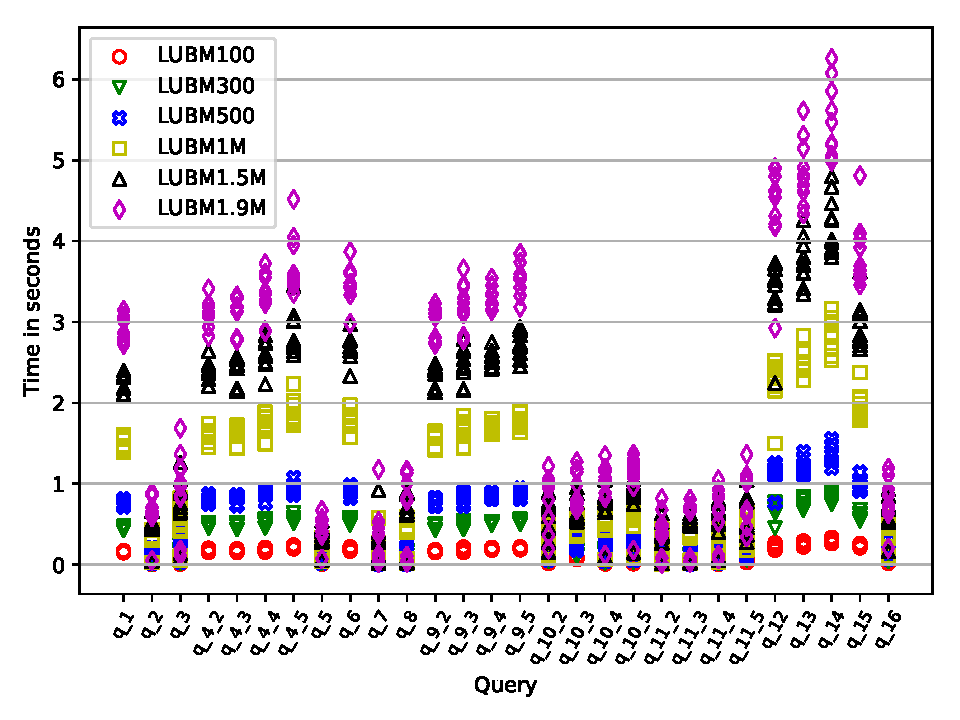
\includegraphics[width=0.48\textwidth]{data/LUBM_all.pdf}
   \caption{Reachability index creation time for LUBM graphs}
   \label{fig:lubm_all_qs}
\end{figure}

Reachability index creation time for each query for for real-world graphs is presented in figure~\ref{fig:other_all_qs}.
We can see that query evaluation time depends on graph inner structure. 
First of all, in some cases handling of small graph requires more time, then handling bigger graph.
For example, $Q_{10}^4$: querying the \textit{geospecies} graph (450k vertices) in some cases requires more time than querying of \textit{mappingbased\_properties} (8.3M vertices) and \textit{taxonomy} (5.7M vertices).
On the other hand, \textit{taxonomy} querying in relatively big number of cases requires significantly more time, than querying of other graphs, while \textit{taxonomy} is not a biggest graph. 
Finally, we can see, that in big number of cases query execution time requires less then 10 seconds, even for big graph, and no queries which require more then 52.17 seconds. 

\begin{figure}
   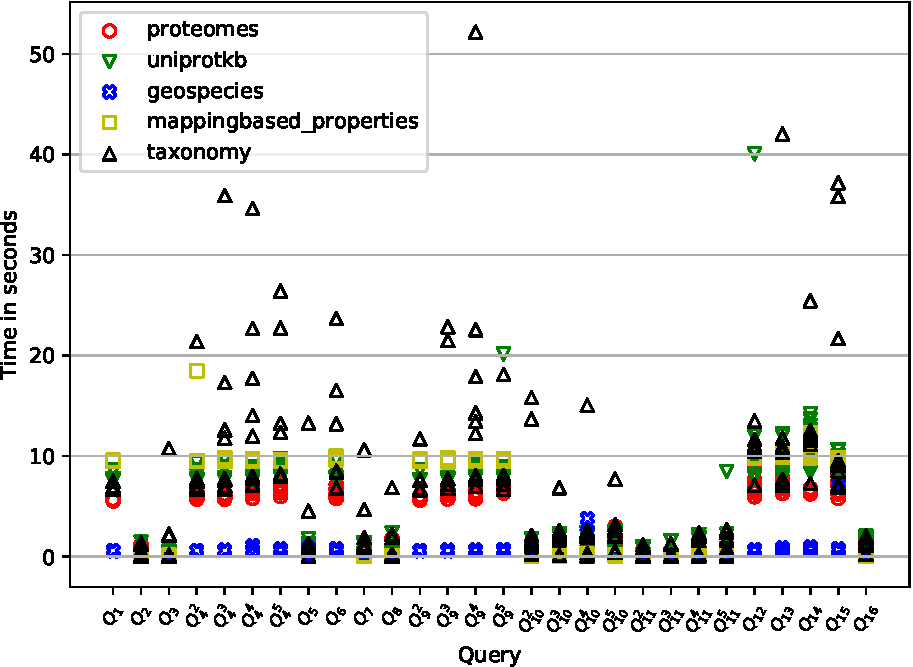
\includegraphics[width=0.48\textwidth]{data/other_all.pdf}
   \caption{Reachability index creation time for real-world RDFs}
   \label{fig:other_all_qs}
\end{figure}

Paths extraction was evaluated on cases with possible long paths.
These cases were selected during reachability index creation by using number of iterations in transitive closure evaluation.
For each selected graph and query we measure paths extraction time for each reachable pair, reachability index creation time is not included because exactly the same index, as calculated at the previous step, is used for paths extraction. 

We evaluate two scenarios.
The first one is a single path extraction.
In this case results are represented as a dependency of extraction time on extracted path length.
We can see linear !!!!

The second scenario is many paths extraction.
Here we limit a number of path to extract by !!! 
In this case results are represented as a dependency of extraction time on number of extracted paths.


\begin{figure}
     \begin{subfigure}[b]{0.24\textwidth}
         \centering
         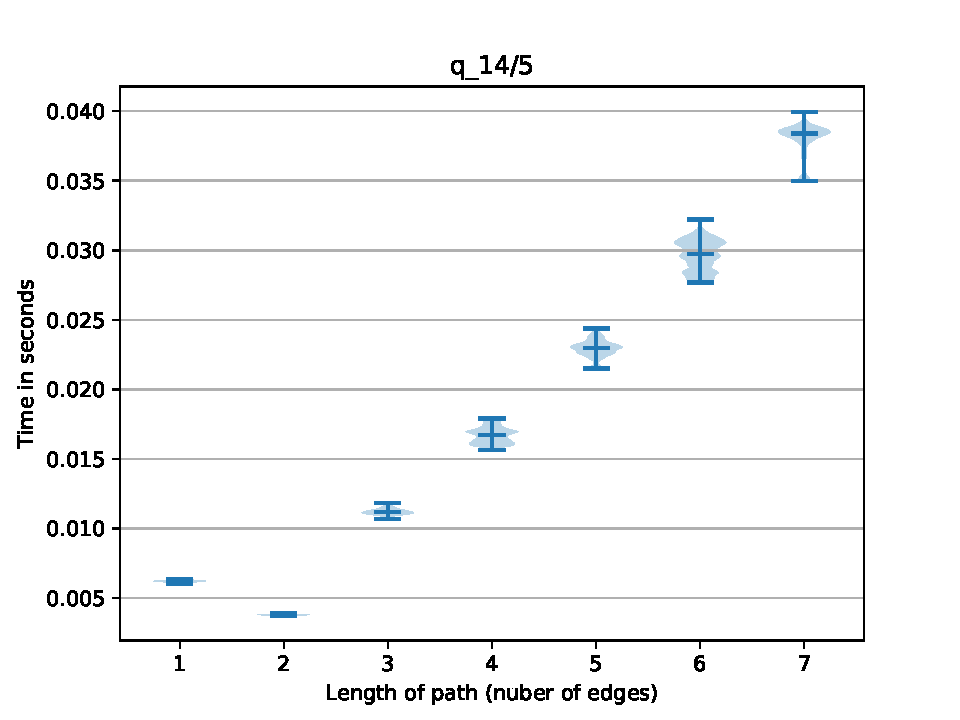
\includegraphics[width=\textwidth]{data/res_graphics/q_14_5.pdf}
         \caption{$y=x$}
         \label{fig:y equals x}
     \end{subfigure}
     ~\begin{subfigure}[b]{0.24\textwidth}
         \centering
         %\includegraphics[width=\textwidth]{data/res_graphics/q9_2_8.pdf}
         \caption{$y=x$}
         \label{fig:y equals x}
     \end{subfigure}\\
     \begin{subfigure}[b]{0.24\textwidth}
         \centering
         %\includegraphics[width=\textwidth]{data/res_graphics/q_14_8.pdf}
         \caption{$y=x$}
         \label{fig:y equals x}
     \end{subfigure}
     ~\begin{subfigure}[b]{0.24\textwidth}
         \centering
         %\includegraphics[width=\textwidth]{data/res_graphics/q4_2_8.pdf}
         \caption{$y=x$}
         \label{fig:y equals x}
     \end{subfigure}
   %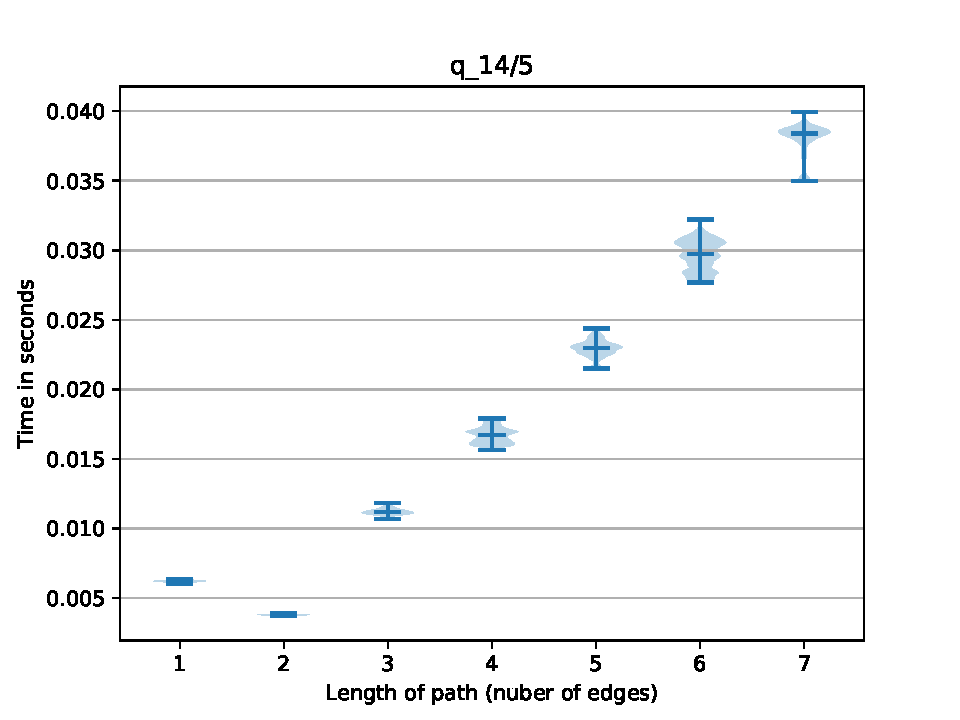
\includegraphics[width=0.48\textwidth]{data/res_graphics/q_14_5.pdf}
   \caption{Single path extraction}
\end{figure}

\subsubsection{Conclusion}

We can conclude that proposed algorithm is applicable for real-world data processing: the algorithm allows one both to solve reachability problem and to extract paths of interest in reasonable time even using na{\"i}ve implementation.  

\subsection{CFPQ Evaluation}

Comparison with matrix-based algorithm.

\subsubsection{Dataset}

Dataset for evaluation. 
It should be CFPQ\_Data\footnote{CFPQ\_Data is a dataset for CFPQ evaluation which contains both synthetic and real-world data and queries \url{https://github.com/JetBrains-Research/CFPQ\_Data}. Access date: 07.07.2020.}

\begin{table}
{
\rowcolors{2}{black!2}{black!10}
\begin{tabular}{|l|c|c|}
\hline
Graph & \#V & \#E \\
\hline
\hline 
eclass\_514en  & 120 926 & 484 646 \\
enzyme  & 358 434 & 144 9711 \\
geospecies  & 596 760 & 2 416 513 \\
go   & 1 188 340 & 4 820 728 \\
go-hierarchy & 1 780 956 & 7 228 358 \\
taxonomy & 2 308 385 & 9 369 511 \\
\hline
Aliases 1 & 6 442 630 & 24 465 430 \\
Aliases 2 & 4 834 262 & 12 366 973 \\
.... & 5 728 398 & 14 922 125 \\
\hline
\end{tabular}
}
\caption{Graphs for CFPQ evaluation}
\label{tbl:graphs_for_cfpq}
\end{table}



Same-generation queries, memory aliases.

\subsubsection{Results}

Results of evaluation.

Index creation.

{\setlength{\tabcolsep}{0.4em}
	\begin{table}
		\caption{RDFs query $G_1$ and $G_2$ (time is measured in seconds and memory is measured in megabytes)}
		\label{tbl:tableRDFQ1_appendix}
		\rowcolors{4}{black!2}{black!10}
		\small
		\begin{tabular}{| l | c | c | c | c |}
			\hline
			
			\multirow{2}{*}{Name}  & \multicolumn{2}{c|}{$G_1$} & \multicolumn{2}{c|}{$G_2$} \\
			\cline{2-5}
			                       & Tensors & RG\_CPU\textsubscript{path} & Tensors & RG\_CPU\textsubscript{path}	 \\
			\hline
			\hline
			eclass\_514en   & 0.254   & 0.195   & 0.227 & ...\\
			enzyme          & 0.035   & 0.029   & 0.036 & ...\\
			geospecies      & 0.091   & ...     & 0.001 & ...\\
			go-hierarchy    & 0.186   & 0.976   & 0.293 & ...\\
			go              & 1.676   & 1.286   & 1.368 & ...\\
			pathways        & 0.015   & 0.021   & 0.009 & ...\\
			taxonomy        & 5.366   & .....   & 3.282 & ...\\
			\hline
		\end{tabular}
	\end{table}
}


Paths extraction.

\subsubsection{Conclusion}

\section{Conclusion and future work}
In this paper, we shown how the context-free path query evaluation w.r.t. the relational and the single-path query semantics can be reduced to the calculation of matrix transitive closure. Also, we provided a formal proof of the correctness of the proposed reduction. In addition, we introduced an algorithm for computing this transitive closure, which allows us to efficiently apply GPGPU computing techniques. Finally, we shown the practical applicability of the proposed algorithm by running different implementations of our algorithm on real-world data.

We can identify several open problems for further research. In this paper we have considered only two semantics of context-free path querying but there are other important semantics, such as all-path query semantics~\cite{hellingsPathQuerying} which requires to present all paths for all triples $(A,m,n)$. Context-free path querying implemented with algorithm~\cite{GLL} can answer the queries in all-path query semantics by constructing a parse forest. It is possible to construct a parse forest for a linear input by matrix multiplication~\cite{okhotin_cyk}. Whether it is possible to generalize this approach for a graph input is an open question.

In our algorithm, we calculate the matrix transitive closure naively, but there are algorithms for the transitive closure calculation, which are asymptotically more efficient. Therefore, the question is whether it is possible to apply these algorithms for the matrix transitive closure calculation to the problem of context-free path querying.

Also, there are Boolean grammars~\cite{okhotinBoolean}, which have more expressive power than context-free grammars. Boolean path querying is an undecidable problem~\cite{hellingsRelational} but our algorithm can be trivially generalized to work on boolean grammars because parsing with boolean grammars can be expressed by matrix multiplication~\cite{okhotin_cyk}. It is not clear what a result of our algorithm applied to Boolean grammars would look like. Our hypothesis is that it would produce the upper approximation of a solution.

From a practical point of view, matrix multiplication in the main loop of the proposed algorithm may be performed on different GPGPU independently. It can help to utilize the power of multi-GPU systems and increase the performance of context-free path querying.

There is an algorithm~\cite{apspGPU} for transitive closure calculation on directed graphs which generalized to handle graph sizes inherently larger then the DRAM memory available on the GPU. Therefore, the question is whether it is possible to apply this approach to the matrix transitive closure calculation in the problem of context-free path querying.

\setmonofont[Mapping=tex-text]{CMU Typewriter Text}
\bibliographystyle{ugost2008ls}
\bibliography{diploma.bib}
\end{document}
